% Edit by 汤
\setcounter{chapter}{5}

\chapter{参数估计\label{cha:6}} % p285

这里所指的参数是指如下三类未知参数:
\begin{itemize}
\item 分布中所含有未知参数 $\theta$. 如: 二点分布 $b(1,p)$ 中的 $p$; 正态分布 $N(\mu,\sigma)$ 中的 $\mu$ 和 $\sigma^2$.
\item 分布中所含的未知参数 $\theta$ 的函数. 如: 服从正态分布 $N(\mu,\sigma^2)$ 的变量 $X$ 不超过某给定值 $a$ 的概率 $P(X\leqslant a)=\Phi\big(\frac{a-\mu}{\sigma}\big)$ 是未知参数 $\mu,\sigma$ 的函数; 单位产品的缺陷数 $X$ 通常服从泊松分布 $P(\lambda)$, 则单位产品合格(无缺陷)的概率 $P(X=0)=\ee^{-\lambda}$ 是未知参数 $\lambda$ 的函数.
\item 分布的各种特征数也都是未知参数, 如: 均值 $E(X)$, 方差 $\mathrm{Var}(X)$,分布中位数等.
\end{itemize}

一般场合,常用日表示参数, 参数 $\theta$ 所有可能取值组成的集合称为参数空间,常用 $\theta$ 表示. 参数估计问题就是根据样本对上述各种未知参数作出估计.

参数估计的形式有两种: 点估计与区间估计. 这里我们从点估计开始.

设 $x_1,x_2,\cdots,x_n$ 是来自总体的一个样本, 我们用一个统计量 $\bar{\theta}=\bar{\theta}(x_1,\cdots,x_n)$ 的取值作为 $\theta$ 的估计值, $\bar{\theta}$ 称为 $\theta$ 的点估计(量), 简称估计. 在这里如何构造统计量并没有明确的规定, 只要它满足一定的合理性即可, 这就涉及两个问题:

\begin{itemize}
\item 其一是如何给出估计, 即估计的方法问题:
\item 其二是如何对不同的估计进行评价, 即估计的好坏判断标准.
\end{itemize}

接下来我们先介绍一些估计的方法, 接着讨论估计的好坏标准, 然后对几个有用的专题给介绍,最后讲述区间估计.

\section{点估计的几种方法\label{section-6-1}} %

人们可以运用各种方法构造出很多 $\theta$ 的估计, 本节介绍两种最常用的点估计方法,它们是: 矩法和最大似然法.

\subsection{替换原理和矩法估计} %6.1.1录入完毕,待检查

1900 年英国统计学家 K.Pearson 提出了一个替换原则, 后来人们称此方法为矩法.

\subsubsection{矩法估计}
%一、矩法估计 P286

替换原理常指如下两句话:
\begin{itemize}
\item 用样本矩去替换总体矩, 这里的矩可以是原点矩也可以是中心矩;
\item 用样本矩的函数去替换相应的总体矩的函数.
\end{itemize}

根据这个替换原理, 在总体分布形式未知场合也可对各种参数作出估计, 譬如:
\begin{itemize}
\item 用样本均值 $\bar{x}$ 估计总体均值 $E(X)$,即 $\hat{E}(X)=\bar{x}$;
\item 用样本方差 $s_n^2$ 品估计总体方差 $\mathrm{Var}(x)$, 即 $\mathrm{\hat{V}ar}(x)=s_n^2$;
\item 用事件 $A$ 出现的频率估计事件 $A$ 发生的概率;
\item 用样本的 $p$ 分位数估计总体的 $p$ 分位数, 特别, 用样本中位数估计总体中位数.
\end{itemize}

\begin{example}
对某型号的 $20$ 辆汽车记录其每 $5L$ 汽油的行驶里程(公里), 观测数据如下:

\begin{tabular}{cccccccccc}
29.8 & 27.6 & 28.3 & 27.9 & 30.1 & 28.7 & 29.9 & 28.0 & 27.9 & 28.7\\
28.4 & 27.2 & 29.5 & 28.5 & 28.0 & 30.0 & 29.1 & 29.8 & 29.6 & 26.9		
\end{tabular}

这是一个容量为 $20$ 的样本观测值, 对应总体是该型号汽车每 $5L$ 汽油的行驶里程, 其分布形式尚不清楚, 可用矩法估计其均值、方差和中位数等. 本例中经计算有
\[\bar{x}=28.695,\quad s_n^2=0.9185,\quad m_{0.5}=28.6,\]
由此给出总体均值、方差和中位数的估计分别为 28.695, 0.9185 和 28.6.
\end{example}

矩法估计的统计思想(替换原理)十分简单明确, 众人都能接受, 使用场合甚广它的实质是用经验分布函数去替换总体分布, 其理论基础是格里纹科定理.

\subsubsection{概率函数 $p(x;\theta)$ 已知时未知参数的矩法估计}

设总体具有已知的概率函数 $p(x;\theta_1,\cdots,\theta_k)$, $(\theta_1,\cdots,\theta_k)\in \Theta$ 未知参数或参数向量,  $x_1,\cdots,x_n$ 是样本, 假定总体的 $k$ 阶原点矩 $\mu_k$ 存在, 则对所有的 $j$,
$0<j<k$, $A$ 内都存在, 若假设 $\theta_1,\cdots,\theta_k$. 能够表示成 $u_1,\cdots,u_k$ 的函数 $\theta_j=\theta_j(u_1,\cdots,u_k)$, 则可给出诸 $\theta_j$ 的矩法估计:
\begin{equation}
\hat{\theta}_j=\theta_j(a_1,\cdots,a_k),\quad j=1,\cdots,k,
\end{equation}
其中 $a_1,\cdots,a_k$. 是前个样本原点矩: $a_j=\frac{1}{n}\sum_{i=1}^{n}x_i^j$. 进一步, 如果我们要估计 $\theta_1,\cdots,\theta_k$
的函数 $\eta=g(\theta_1,\cdots,\theta_k)$, 则可直接得到 $\eta$ 的矩法估计
\begin{equation}
\hat{\eta}=g(\hat{\theta}_1,\cdots,\hat{\theta}_k),
\end{equation}
当 $k=1$ 时, 我们通常可以由样本均值出发对未知参数进行估计; 如果 $k=2$, 我们可以由一阶、二阶原点矩(或二阶中心矩)出发估计未知参数.

\begin{example}
设总体为指数分布, 其密度函数为
\[p(x;\lambda)=\lambda\cdot\ee^{-\lambda x},\quad x>0, \]
$x_1,\cdots,x_n$ 是样本, 此处 $k=1$, 由于 $EX=1/\lambda$, 亦即 $\lambda=1/EX$, 故 $\lambda$ 的矩法估计为
\[\hat{\lambda}=1/\bar{x}. \]
另外, 由于 $\mathrm{Var}(X)=1/\lambda^2$, 其反函数为 $\lambda=1/\sqrt{\mathrm{Var}(X)}$, 因此, 从替换原理来看, $\lambda$ 的矩法估计也可取为
\[\hat{\lambda}_1=1/s. \]
$s$为样本标准差. 这说明矩估计可能是不唯一的, 这是矩法估计的一个缺点, 此时通常应该尽量采用低阶矩给出未知参数的估计.
\end{example}

\begin{example}
$x_1,\cdots,x_n$ 是来自 $(a,b)$ 上的均匀分布 $U(a,b)$ 的样本, $a$ 与 $b$ 均是未知参数, 这里 $k=2$, 由于
\[EX=\frac{a+b}{2},\quad\mathrm{Var}(X)=\frac{(b-a)^2}{12}, \]
不难推出
\[a=EX-\sqrt{3\mathrm{Var}(X)},\quad b=EX+\sqrt{3\mathrm{Var}(X)}, \]
由此即可得到 $a,b$ 的矩估计:
\[\hat{a}=\bar{x}-\sqrt{3}s,\quad\hat{b}=\bar{x}+\sqrt{3}s, \]
若从均匀总体 $U(a,b)$ 获得如下一个容量为 5 的样本: $4.5\quad5.0\quad4.7\quad4.0\quad4.2$, 经计算, 有 $\bar{x}=4.48,s_n=0.3962$, 于是可得 $a,b$ 的矩估计为
\[\hat{a}=4.48-0.3962\sqrt{3}=3.7938,\]
\[\hat{b}=4.48+0.3962\sqrt{3}=5.1662.\]
\end{example}

\subsection{最大似然估计}%6.1.2录入完毕,待检查

最大似然估计法是求估计用得最多的方法, 它最早是由高斯在 1821 年提出, 但一般将之归功于费希尔(R.A.Fisher), 因为费希尔在 1922 年再次提出了这种想法并证明了它的一些性质而使得最大似然法得到了广泛的应用.

为了叙述最大似然原理的直观想法, 先看两个例子.

\begin{example}
设有外形完全相同的两个箱子, 甲箱中有 99 个白球和 1 个黑球, 乙箱中有 99 个黑球和 1 个白球, 今随机地抽取一箱, 并从中随机抽取一球, 结果取得白球, 间这球是从哪一个箱子中取出?
\end{example}
\begin{solution}
不管是哪一个箱子, 从箱子中任取一球都有两个可能的结果:$A$ 表示取出白球,$B$ 表示取出黑球. 如果我们取出的是甲箱, 则 $A$ 发生的概率为 0.99, 而如果取出的是乙箱, 则 $A$ 发生的概率为 0.01. 现在一次试验中结果 $A$ 发生了, 人们的第一印象就是: “此白球 $(A)$ 最像从甲箱取出的”, 或者说, 应该认为试验条件对结果 $A$ 出现有利,从而可以推断这球是从甲箱中取出的. 这个推断很符合人们的经验事实, 这里 “最像” 就是 “最大似然” 之意.

本例中假设的数据很极端. 一般地, 我们可以这样设想: 有两个箱子中各有 100 只球,甲箱中白球的比例是 $p_1$, 乙箱中白球的比例是 $p_2$, 已知 $p_1>p_2$, 现随即地抽取一个箱子并从中抽取一球, 假定取到的是白球, 如果我们要在两个箱子中进行选择, 由子甲箱中白球的比例高于乙箱, 根据最大似然原理, 我们应该推断该球来自甲箱.
\end{solution}

\begin{example}\label{exam:6.1.5}
设产品分为合格品与不合格品两类, 我们用一个随即变量 $X$ 来表示某个产品是否合格, $X=0$ 表示合格品, $X=1$ 表示不合格品, 则 $X$ 服从二点分布 $b(1,p)$, 其中 $p$ 是未知的不合格品率. 现抽取 $n$ 个产品看其是否合格, 得到样本 $x_1,\cdots,x_n$, 这批观测值发生的概率为:
\begin{equation}\label{eq:6.1.3}
P(X_1=x_1,\cdots,X_n=x_n;p)=\prod_{i=1}^np^{x_i}(1-p)^{1-x_i}=p^{\sum x_i}(1-p)^{n-\sum x_i}, %6.1.3
\end{equation}
由子 $p$ 是未知的, 根据最大似然原理, 我们应选择 $p$ 使得 \eqref{eq:6.1.3} 表示的概率尽可能大. 将\eqref{eq:6.1.3}看作未知参数 $p$ 的函数,用 $L(p)$ 表示, 称作\textbf{似然函数}\index{C!参数估计!似然函数}, 亦即
\begin{equation}\label{eq:6.1.4}
L(p)=p^{\sum x_i}(1-p)^{n-\sum x_i},
\end{equation}
要求 \eqref{eq:6.1.4} 的最大值点不是难事, 将 \eqref{eq:6.1.4} 两端取对数并关子 $p$ 求导令其为 $\Theta$, 即得如下方程:
\begin{equation}\label{eq:6.1.5}
\frac{\partial \ln L(p)}{\partial p}=\frac{\sum x_i}{p}-\frac{n-\sum x_i}{1-p}=0
\end{equation}
解之即得 $p$ 的最大\textbf{似然估计}\index{C!参数估计!似然估计}, 为
\[\hat{p}=\hat{p}(x_1,\cdots,x_n)=\sum x_i/n=\bar{x}. \]
由例\ref{eq:6.1.5} 我们可以看到求最大似然估计的基本思路, 对离散型总体, 设有样本观测值 $x_1,\cdots,x_n$, 我们写出该观测值出现的概率, 它一般依赖子某个或某些参数, 用 $\theta$ 表示,将该概率看成 $\theta$ 的函数, 用 $L(\theta)$ 表示, 即
\[L(\theta)=L(X_1=x_1,\cdots,X_n=x_n;\theta), \]
求最大似然估计就是找 $\theta$ 的估计值 $\hat{\theta}=\hat{\theta}(x_1,\cdots,x_n)$ 使得上式的 $L(\theta)$ 达到最大.
\end{example}

对连续型总体, 样本观测值 $x_1,\cdots,x_n$ 出现的概率总是为 0 的, 但我们可用联合概率密度函数来表示随机变量在观测值附近出现的可能性大小, 也将之称为似然函数, 由此, 我们给出如下正规的定义.

\begin{definition}{}{}%6.1.1
设总体的概率函数为 $p(x;\theta)$, $\theta\in\Theta$, 日,其中 $\theta$ 是一个未知参数或几个未知参数组成的参数向量, 是参数 $\theta$ 可能取值的参数空间, $x_1,\cdots,x_n$ 是来自该总体的样本, 将样本的联合概率函数看成8的函数,用 $L(\theta;x_1,\cdots,x_n)$ 表示, 简记为 $L(\theta)$,
\begin{equation}\label{eq:6.1.6}
L(\theta)=L(\theta;x_1,\cdots,x_n)=p(x_1;\theta)\cdot p(x_2;\theta)\cdot \cdots \cdot p(x_n;\theta),
\end{equation}
$L(\theta)$ 称为样本的似然函数. 如果某统计量 $\hat{\theta}=\hat{\theta}(x_1,\cdots,x_n)$ 满足
\begin{equation}\label{eq:6.1.7}
L(\hat{\theta})=\max_{\theta\in\Theta}L(\theta),
\end{equation}
则称 $\hat{\theta}$ 是 $\theta$ 的\textbf{最大似然估计}\index{C!参数估计!最大似然估计}, 简记为 MLE(Maximum Likelihood Estimate).
\end{definition}

由于 $\ln x$ 是 $x$ 的单调增函数, 因此, 使对数似然函数 $\ln L(\theta)$ 达到最大与使 $L(\theta)$ 达到最大是等价的. 人们通常更习惯于由 $\ln L(\theta)$ 出发寻找日的最大似然估计. 当 $L(\theta)$ 是可微函数时, 求导是求最大似然估计最常用的方法,此时对对数似然函数求导更加简单些.

\begin{example}
设一个试验有三种可能结果,其发生概率分别为
\begin{equation}\label{eq:6.1.8}
p_1=\theta^2,\quad p_2=2\theta(1-\theta),\quad p_3=(1-\theta)^2.
\end{equation}
现做了 $n$ 次试验,观测到三种结果发生的次数分别为 $n_1,n_2,n_3(n_1+n_2+n_3=n)$. 则似然函数为
\begin{align*}
L(\theta)
&=\big(\theta^{2}\big)^{n_1}[2 \theta(1-\theta)]^{n_{2}}\left[(1-\theta)^{2}\right]^{n_{3}} \\ &=2^{n_{2}} \theta^{2 n_{1}+n_{2}}(1-\theta)^{2 n_{3}+n_{2}}
\end{align*}
其对数似然函数为
\[\ln L(\theta)=\left(2 n_{1}+n_{2}\right)\ln\theta+\left(2 n_{3}+n_{2}\right)\ln (1-\theta)+n_{2}\ln 2,\]
将之关于 $\theta$ 求导并令其为 0 得到似然方程
\[\frac{2 n_{1}+n_{2}}{\theta}-\frac{2 n_{3}+n_{2}}{1-\theta}=0,\]
解之,得
\[\hat{\theta}=\frac{2 n_{1}+n_{2}}{2\left(n_{1}+n_{2}+n_{3}\right)}=\frac{2 n_{1}+n_{2}}{2 n},\]
由于
\[\frac{\partial^{2} \ln L(\theta)}{\partial \theta^{2}}=-\frac{2 n_{1}+n_{2}}{\theta^{2}}-\frac{2 n_{3}+n_{2}}{(1-\theta)^{2}}<0,\]
所以 $\hat{\theta}$ 是极大值点.
\end{example}

\begin{example}\label{exam:6.1.7}
对正态总体 $N(u,\delta^2)$, $\theta=(u,\delta^2)$ 是二维参数, 设有样本 $x_1,\cdots,x_n$, 则似然函数及其对数分别为
\begin{align*}
L\left(\mu,\sigma^{2}\right)
&=\prod_{i=1}^{n}\left\{\frac{1}{\sqrt{2\pi}\sigma}\exp \left\{-\frac{\left(x_{i}-\mu\right)^{2}}{2 \sigma^{2}}\right\}\right\}\\
&=\left(2\pi\sigma^{2}\right)^{-n/2}\exp\left\{-\frac{1}{2 \sigma^{2}}\sum_{i=1}^{n}\left(x_{i}-\mu\right)^{2}\right\}
\end{align*}
\[\ln L\left(\mu,\sigma^{2}\right)=-\frac{1}{2\sigma^{2}} \sum_{i=1}^{n}\left(x_{i}-\mu\right)^{2}-\frac{n}{2} \ln \sigma^{2}-\frac{n}{2}\ln(2\pi)\]
将 $\ln L(\mu,\delta^2)$ 分别关于两个分量求偏导并令其为 0 即得到似然方程组
将 $\ln L(u,\delta^2)$ 分别关于两个分量求偏导并令其为 0 即得到似然方程组
\begin{equation}\label{eq:6.1.9}
\frac{\partial\ln L\left(\mu, \sigma^{2}\right)}{\partial \mu}=\frac{1}{\sigma^{2}} \sum_{i=1}^{n}\left(x_{i}-\mu\right)=0
\end{equation}
\begin{equation}\label{eq:6.1.10}
\frac{\partial \ln L\left(\mu, \sigma^{2}\right)}{\partial \sigma^{2}}=\frac{1}{2 \sigma^{4}} \sum_{i=1}^{n}\left(x_{i}-\mu\right)^{2}-\frac{n}{2\sigma^{2}}=0
\end{equation}
解此方程组, 由 \eqref{eq:6.1.9} 可得 $\mu$ 的最大似然估计为
\[\hat{\mu}=\frac{1}{n} \sum_{z=1}^{n} x_{i}=\overline{x},\]
将之代入 \eqref{eq:6.1.10} 给出 $\delta^2$ 的最大似然估计
\[\vec{\sigma}^{2}=\frac{1}{n} \sum_{i=1}^{n}\left(x_{i}-\overline{x}\right)^{2}=s^{* 2},\]
利用二阶导函数矩阵的非正定性可以说明上述估计使得似然函数取极大值.

虽然求导函数是求最大似然估计最常用的方法, 但并不是在所有场合求导都是有效的, 下面的例子说明了这个问题.
\end{example}

\begin{example}%6.1.8
设 $x_1,\cdots,x_n$ 是来自均匀总体 $U(0,\theta)$ 的样本, 试求 $\theta$ 的最大似然估计.
\end{example}
\begin{solution}
似然函数
\[L(\theta)=\frac{1}{\theta^n}\prod_{i=1}^nI_{\{0<X_i\leqslant\theta\}}=\frac{1}{\theta^n}I_{\{X_{(n)}\leqslant\theta\}} \]
要使 $L(\theta)$ 达到最大, 首先一点是示性函数取值应该为 1, 其次是 $1/\theta^n$ 尽可能大. 由于 $1/\theta^n$ 是 $\theta$ 的单调减函数, 所以 $\theta$ 的取值应尽可能小, 但示性函数为 1 决定了 $\theta$ 不能小于x(a), 由此给出 $\theta$ 的最大似然估计: $\hat{\theta}=x_{(n)}$.

最大似然估计有一个简单面有用的性质: 如果是 $\theta$ 的最大似然估计, 则对任一函数 $g(\theta)$, 其最大似然估计为 $g(\hat{\theta})$. 该性质称为最大似然估计的不变性, 从而使一些复杂结构的参数的最大似然估计的获得变得容易了.
\end{solution}

\begin{example}
设 $x_1,\cdots,x_n$ 是来自正态总体 $N(\mu,\delta^2)$ 的样本, 在例\ref{exam:6.1.7}中已求得 $\mu$ 和 $\delta^2$ 的最大似然估计为
\[\hat{\mu}=\overline{x},\quad\hat{\sigma}^{2}=s^{*2}\]
于是由最大似然估计的不变性可得如下参数的最大似然估计, 它们是
\begin{itemize}
\item 标准差 $\delta$ 的MLE是 $\delta=\sigma^*$;
\item 概率 $P(X<3)=\Phi\big(\frac{3-u}{\delta}\big)$ 的 MLE 是 $\Phi\big(\frac{3-\bar{x}}{s^*}\big)$;
\item 总体 0.90 分位数 $x_{0.90}=\mu+\sigma\cdot\mu_{0.90}$ 的 MLE 是 $\bar{x}+s^{*}\cdot u_{0.90}$, 其中 $u_{0.90}$ 为标准正态分布的 0.90 分位数.
\end{itemize}
\end{example}



\begin{xiti}
\item 从一批电子元件中抽取 8 个进行寿命测试, 得到如下数据 (单位:h):
\begin{center}
\begin{tabular}{cccccccc}
	1050,&1100,&1130,&1040,&1250,&1300,&1200,&1080
\end{tabular}
\end{center}
试对这批元件的平均寿命以及寿命分布的标准差给出矩估计.
\item 设总体 $X\sim U(0,\theta)$, 现从该总体中抽取容量为 10 的样本, 样本值为:
\begin{center}
\begin{tabular}{cccccccccc}
0.5,&1.3,&0.6,&1.7,&2.2,&1.2,&0.8,&1.5,&2.0,&1.6
\end{tabular}	
\end{center}
试对参数 $\theta$ 给出矩估计.
\item 设总体分布列如下, $x_1,x_2,\cdots,x_n$ 是样本, 试求未知参数的矩估计.
\begin{enumerate}
\item $P(X=k)=\frac{1}{N}, k=0,1,2, \cdots, N-1, N$, (正整数)是未知参数;
\item  $P(X=k)=(k-1) \theta^{2}(1-\theta)^{k-2}, k=2,3, \cdots, 0<\theta<1$.
\end{enumerate}

\item 设总体密度函数如下, $x_1,x_2,\cdots,x_n$ 是样本, 试求未知参数的矩估计. 
\begin{enumerate}
  \item $p(x ; \theta)=\frac{2}{\theta^{2}}(\theta-x), 0<x<\theta, \theta>0$, 
  \item $p(x ; \theta)=(\theta+1) x^{8}, 0<x<1, \theta>0$, 
  \item $p(x ; \theta)=\sqrt{\theta} x^{\sqrt8-t}, 0<x<1, \theta>0$, 
  \item $p(x ; \theta, \mu)=\frac{1}{\theta} \mathrm{e}^{-\frac{x-\mu}{\theta}}, x>\mu, \theta>0$.
\end{enumerate}

\item 设总体为 $N(\mu,1)$, 现对该总体观测 $n$ 次, 发现有 $k$ 次观测值为正, 使用频率替换方法求 $A$ 的估计.
\item 甲、乙两个校对员被此独立对同一本书的样稿进行校对, 校完后, 甲发现 $a$ 个错字, 乙发现 $b$ 个错字, 其中共同发现的错字有 $c$ 个, 试用矩法给出如下两个未知参数的估计:
\begin{enumerate}
  \item 该书样稿的总错字个数;
  \item 未被发现的错字数.
\end{enumerate}

\item 设总体概率函数如, $x_1,x_2,\cdots,x_n$ 是样本, 试求未知参数的最大似然估计. 
\begin{enumerate}
  \item $p(x ; \theta)=\sqrt{\theta} x^{\sqrt{\theta}-1}, 0<x<1, \theta>0$, 
  \item $p(x ; \theta)=\theta c^{\theta} x^{-(\theta+1)}, x>c, c>0$, 已知,  $\theta>1$.
\end{enumerate}

\item 设总体概率函数如下, $x_1,x_2,\cdots,x_n$ 是样本, 试求未知参数的最大似然估计.
\begin{enumerate}
  \item $p(x ; \theta)=c \theta^{c} x^{-(c+1)}, x>\theta, \theta>0, c>0$已知 ,
  \item $p(x ; \theta, \mu)=\frac{1}{\theta} e^{-\frac{x-\mu}{\theta}}, x>\mu, \theta>0$ ,
  \item $p(x ; \theta)=(k \theta)^{-1}, \theta<x<(k+1) \theta, \theta>0$ .
\end{enumerate}

\item 设总体概率函数如下, $x_1,x_2,\cdots,x_n$ 是样本, 试求未知参数的最大似然估计.
\begin{enumerate}
  \item $p(x ; \theta)=\frac{1}{2\theta} \ee^{-|x| / \theta}, \theta>0$ ,
  \item $p(x ; \theta)=1, \theta-1 / 2<x<\theta+1 / 2$ ,
  \item $p\left(x ; \theta_{1}, \theta_{2}\right)=\frac{1}{\theta_{2}-\theta_{1}}, \theta_{1}<x<\theta_{2}$ .
\end{enumerate}
\item 一地质学家为研究密歇根湖的湖滩地区的岩石成分, 随机地自该地区取 100 个样品,每个样品有 10 块石子, 记录了每个样品中属石灰石的石子数. 假设这 100 次观豪相互独立, 求这地区石子中石灰石的比例 $p$ 的最大似然估计.该地质学家所得的数据如下:
\begin{center}
\begin{tabularx}{0.8\textwidth}{Z|*{10}{c|}c}
样本中的石子数 & 0 & 1 & 2 & 3 & 4 & 5 & 6 & 7 & 8 & 9 & 10\\
\midrule
样品个数 & 0 & 1 & 6 & 7 & 23 & 26 & 21 & 12 & 3 & 1 & 0
\end{tabularx}
\end{center}

\item 在遗传学研究中经常要从截尾二项分布中抽样,其总体概率函数为
\[P\left(X=k; p\right)=\frac{\binom mk p^{k}(1-p)^{m-k}}{1-(1-p)^{m}}, k=1,2, \cdots, m\]
若已知 $m=2$, $x_1,x_2,\cdots,x_n$ 是样本,试求 $p$ 的最大似然估计.

\item 已知在文学家萧伯纳的 “An Intelligent Woman's Guide To Socialism”一书中, 一个句子的单词数 $X$ 近似地服从对数正态分布, 即 $x=\ln X\sim N(\mu,\sigma^2)$. 今从该书中随机地取 20 个句子, 这些句子中的单词数分别为
\begin{center}
\begin{tabularx}{0.8\textwidth}{*{10}{Z}}
52 & 24 & 15 & 67 & 15 & 22 & 63 & 26 & 16 & 32\\
7 & 33 & 28 & 14 & 7 & 29 & 10 & 6 & 59 & 30
\end{tabularx}	
\end{center}
求该书中一个句子单词数均值 $E(X)=\ee^{\mu+\sigma^2/2}$ 的最大似然估计.
\end{xiti}

\section{点估计的评价标准}\label{sec:6.2}

我们已经看到,点估计有各种不同的求法, 为了在不同的点估计间进行比较选择, 就必须对各种点估计的好坏给出评价标准.

数理统计中给出了众多的估计量评价标准,对同一估计量使用不同的评价标准可能会得到完全不同的结论, 因此, 在评价某一个估计好坏时首先要说明是在哪一个标准下, 否则所论好坏则毫无意义.

但不管怎么说, 有一个基本标准是所有的估计都应该满足的, 它是衡量一个估计是否可行的必要条件, 这就是估计的相合性, 我们就从相合性开始.

\subsection{相关性}\label{ssec:6.2.1} % P293 录入完毕,未检查

\begin{definition}{}{6.2.1}
设 $\theta\in\Theta$ 为未知参数, $\hat{\theta}_n=\hat{\theta}_n(x_1,\cdots,x_n)$ 是 $\theta$ 的一个估计量, $n$ 是样本容量, 若对任何一个 $\varepsilon>0$, 有
\begin{equation}\label{eq:6.2.1}
\lim _{n \rightarrow \infty} P(|\hat{\theta}_{n}-\theta|>\varepsilon)=0
\end{equation}
则称 $\hat{\theta}_n$ 为参数 $\theta$ 的相合估计.
\end{definition}
相合性被认为是对估计的一个最基本要求, 如果一个估计量, 在样本量不断增大时, 它都不能把被估参数估计到任意指定的精度, 那么这个估计是很值得怀疑的. 通常, 不满足相合性要求的估计一般不予考虑. 证明估计的相合性一般可应用大数定律或直接由定义来证.

若把依赖于样本量 $n$ 的估计量 $\hat{\theta}_n$. 看作一个随机变量序列, 相合性就是 $\hat{\theta}_n$. 依概率收敛于 $\theta$,所以证明估计的相合性可应用依概率收敛的性质及各种大数定律.

\begin{example}\label{exam:6.2.1}
设 $x_1,\cdots,x_n$ 是来自正态总体 $N(\mu,\sigma^2)$ 的样本,则由辛钦大数定律及依概率收敛的性质知:
\begin{itemize}
\item $\bar x$ 是 $\mu$ 的相合估计;
\item $s^{*2}$ 是 $\sigma^2$ 的相合估计;
\item $s^2$ 也是 $\sigma^2$ 的相合估计.
\end{itemize}
由此可见参数的相合估计不止一个.
\end{example}

\begin{theorem}{}{6.2.1}
设 $\hat{\theta}_n=\hat{\theta}_n(x_1,\cdots,x_n)$ 是 $\theta$ 的一个估计量, 若
\begin{equation}\label{eq:6.2.2}
\lim _{n \rightarrow+\infty} E(\hat{\theta}_{n})=\theta, \quad \lim _{n \rightarrow+\infty} \operatorname{Var}(\hat{\theta}_{n})=0
\end{equation}
则 $\hat{\theta}_n$ 是 $\theta$ 的相合估计,
\end{theorem}\begin{proof}
对任意的 $\varepsilon>0$, 由切比雪夫不等式有
\[P(|\hat{\theta}_{n}-E \hat{\theta}_{n}| \geqslant \varepsilon / 2) \leqslant \frac{4}{\varepsilon^{2}} \operatorname{Var}(\hat{\theta}_{n})\]
另一方面,由 $\lim _{n \rightarrow+\infty} E(\hat{\theta}_{n})=\theta$ 可知, 当 $n$ 充分大时有
\[|E \hat{\theta}_{n}-\theta|<\varepsilon / 2\]
注意到此时如果 $|\hat{\theta}_n-E\hat{\theta}_n|<\varepsilon/2$, 就有
\[|\hat{\theta}_{n}-\theta| \leqslant|\hat{\theta}_{n}-E \hat{\theta}_{n}|+|E \hat{\theta}_{n}-\theta|<\varepsilon\]
故
\[\{|\hat{\theta}_{n}-E \hat{\theta}_{n}|<\varepsilon / 2\} \subset| | \hat{\theta}_{n}-\theta |<\varepsilon \}\]
等价地
\[\{ | \hat{\theta}_{n}-E \hat{\theta}_{n}|< \varepsilon/ 2 \} \supset\{|\hat{\theta}_{n}-\theta|<\varepsilon \}\]
由此即有
\[P(|\hat{\theta}_{n}-\theta|>\epsilon) \leqslant P(|\hat{\theta}_{n}-E \hat{\theta}_{n}| \geqslant \epsilon / 2) \leqslant \frac{4}{\varepsilon^{2}} \operatorname{Var}(\hat{\theta}_{n}) \rightarrow 0(n \rightarrow+\infty)\]
定理得证.
\end{proof}

\begin{example}\label{exam:6.2.2}
设 $x_1,\cdots,x_n$ 是来自均匀总体 $U(0,0)$ 的样本, 证明 $\theta$ 的最大似然估计是相合估计.
\end{example}
\begin{proof}
在例\ref{exam:6.1.7}中我们已经给出 $\theta$ 的最大似然估计是 $x_{(n)}$.  由次序统计量的分布, 我们知道 $\hat{\theta}=x_{(n)}$ 的分布密度函数为
\[p(y)=n y^{n-1} / \theta^{n}, \quad y<\theta\]
故有
\[E \hat{\theta}=\int_{0}^{\theta} n y^{n}\dd y / \theta^{n}=\frac{n}{n+1} \theta \rightarrow \theta\]
\[E \hat{\theta^{2}}=\int_{0}^{\theta} n y^{n+1} \mathrm{d} y / \theta^{n}=\frac{n}{n+2} \theta^{2}\]
\[\operatorname{Var}(\hat{\theta})=\frac{n}{n+2} \theta^{2}-\left(\frac{n}{n+1} \theta\right)^{2}=\frac{n}{(n+1)^{2}(n+2)} \theta^{2} \rightarrow 0 \quad(n \rightarrow+\infty)\]
由定理\ref{thm:6.2.1}可知,  $x_{(n)}$ 是 $\theta$ 的相合估计.
\end{proof}

\begin{theorem}{}{6.2.2} %定理6.2.2 P294
若 $\hat{\theta}_{n1},\cdots,\hat{\theta}_{nk}$ 分别是 $\theta_1,\cdots,\theta_k$ 的相合估计, $\eta=g(\theta_1,\cdots,\theta_k)$ 是 $\theta_1,\cdots,\theta_k$ 的连续函数,则 $\bar{\eta}_n=g(\hat{\theta}_{n1},\cdots,\hat{\theta}_{nk})$ 是 $\eta$ 的相合估计.
\end{theorem}
\begin{proof}
由函数 $g$ 的连续性, 对任意给定的 $\varepsilon>0$, 存在一个 $\delta>0$, 当 $|\hat{\theta}_j-\theta_j|<\delta,j=1,\cdots,k$, 有
\begin{equation}\label{eq:6.2.3}
|g(\hat{\theta}_{1}, \cdots, \hat{\theta}_{k})-g(\theta_{1}, \cdots, \theta_{k})|<\varepsilon
\end{equation}
又由 $\hat{\theta}_{n1},\cdots,\hat{\theta}_{nk}$ 是的相合性, 对给定的 $\delta$, 对任意给定的 $v>0$, 存在正整数 $N$, 使得 $n\geqslant N$ 时,
\[P(|\hat{\theta}_{n j}-\theta_{j}| \geqslant \delta)<v / k, \quad j=1, \cdots, k\]
从而有
\begin{align*}
P\left(\bigcap_{i=1}^{k}\{|\hat{\theta}_{n j}-\theta_{j}|<\delta\}\right)
&=1-P\left(\bigcup_{j=1}^{k}\{ | \vec{\theta}_{n j}-\theta_{j} | \geqslant \delta\}\right)\\
&\geqslant 1-\sum_{j=1}^{k} P(|\hat{\theta}_{n j}-\theta_{j}| \geqslant \delta)\\
&>1-k \cdot v / k=1-v
\end{align*}
根据\eqref{eq:6.2.3}, $\bigcap_{j=1}^{k}\{|\hat{\theta}_{n j}-\theta_{j}|<\delta\} \subset\{ | \hat{\eta}_{n}-\eta |<\varepsilon \}$ 故有
\[P\left(\left|\hat{\eta}_{n}-\eta\right|<\epsilon\right)>1-v\]
由v的任意性,定理得证.
\end{proof}

由大数定律及定理\ref{thm:6.2.2}, 我们可以看到, 矩估计一般都具有相合性. 比如:
\begin{itemize}
\item 样本均值是总体均值的相合估计;
\item 样本标准差是总体标准差的相合估计;
\item 样本变异系数 $s/\bar x$ 是总体变异系数的相合估计.
\end{itemize}

\begin{example}\label{exam:6.2.3}
设一个试验有三种可能结果, 其发生概率分别为
\[p_{1}=\theta^{2}, \quad p_{2}=2 \theta(1-\theta), p_{3}=(1-\theta)^{2}\]
现做了 $n$ 次试验,观测到三种结果发生的次数分别为 $n_1,n_2,n_3$ 可以采用频率替换方法估计 $\theta$. 由于可以有三个不同的日的表达式:
\[\theta=\sqrt{p_{1}}, \quad \theta=1-\sqrt{p_{3}}, \quad \theta=p_{1}+p_{2} / 2\]
从而可以给出 $\theta$ 三种不同的频率替换估计,它们分别是:
\[\hat{\theta}_{1}=\sqrt{n_{1} / n}, \quad \hat{\theta}_{2}=1-\sqrt{n_{3} / n}, \quad \hat{\theta}_{3}=\left(n_{1}+n_{2} / 2\right) / n\]
由大数定律, $n_1/n,n_2/n,n_3/n$ 分别是 $p_1,p_2,p_3$ 的相合估计,由定理\ref{thm:6.2.2}知, 上述三个估计都是 $\theta$ 的相合估计.
\end{example}

\subsection{无偏性}\label{ssec:6.2.2} % P295 录入完毕,未检查

相合性是大样本下估计量的评价标准, 对小样本而言, 需要一些其他的评价标准, 无偏性便是一个常用的评价标准.

\begin{definition}{}{6.2.2} % P295
设 $\hat{\theta}_n=\hat{\theta}_n(x_1,\cdots,x_n)$ 是 $\theta$ 的一个估计, $\theta$ 的参数空间为 $\Theta$ ,若对任意的 $\theta\in\Theta$, 有
\begin{equation}\label{eq:6.2.4}
E(\hat{\theta})=\theta
\end{equation}
则称 $\hat\theta$ 是 $\theta$ 的{\heiti 无偏估计}\index{C!参数估计!无偏估计}, 否则称为{\heiti 有偏估计}\index{C!参数估计!有偏估计}.
\end{definition}

无偏性要求可以改写为 $E(\hat{\theta}-\theta)=0$, 这表示无偏估计没有系统偏差,当我们使用 $\hat{\theta}$ 估计 $\theta$ 时, 由于样本的随机性, $\hat{\theta}$ 与 $\theta$ 总是有偏差的, 这种偏差时而(对某些样本观测值)为正, 时而(对另一些样本观测值)为负, 时而大, 时而小. 无偏性表示, 把这些偏差平均起来其值为 0, 这就是无偏估计的含义. 而若估计不具有无偏性, 则无论使用多少次, 其平均也会与参数真值有一定的距离, 这个距离就是系统误差.

\begin{example}\label{exam:6.2.4}
对任一总体而言, 样本均值是总体均值的无偏估计. 当总体 $k$ 阶矩存在时, 样本 $k$ 阶原点矩 $a_k$ 是总体息 $k$ 阶原点矩 $\mu_k$ 么的无偏估计. 但对 $k$ 阶中心矩则不一样, 譬如, 样本方差 $s^{*2}$ 就不是总体方差 $\sigma^2$ 的无偏估计, 因在定理\ref{thm:5.2.1}
中已经指出:
\[E\left(s^{* 2}\right)=\frac{n-1}{n} \sigma^{2}\]
对此, 有如下两点说明:
\begin{enumerate}
  \item 当样本量趋于无穷时, 有 $E(s^{*2})\to\sigma^2$, 我们称 $s^{*2}$ 为 $\sigma^2$ 的渐近无偏估计, 这表明当样本量较大时,  $s^{*2}$ 可近似看作 $\sigma^2$ 的无偏估计.

  \item 若对 $s^{*2}$ 作如下修正:
\begin{equation}\label{eq:6.2.5}
s^{2}=\frac{n s^{* 2}}{n-1}=\frac{1}{n-1} \sum_{i=1}^{n}\left(x_{i}-\overline{x}\right)^{2}
\end{equation}
则 $s^2$ 是总体方差的无偏估计.这种简单的修正方法在一些场合常被采用.\eqref{eq:6.2.5}定义的 $s^2$ 也称为样本方差,它比 $s^{*2}$ 更常用.这是因为在 $n\geqslant2$ 时,$s^{*2}<s^2$,因此用 $s^{*2}$ 估计 $\sigma^2$ 有偏小的倾向,特别在小样本场合要使用 $s^2$ 估计 $\sigma^2$.
\end{enumerate}

无偏性不具有不变性. 即若 $\hat{\theta}$ 是 $\theta$ 的无偏估计, 一般而言, $g(\hat{\theta})$ 不是 $g(\theta)$ 的无偏估计, 除非 $g(\theta)$ 是 $\theta$ 的线性函数.譬如,$s^2$ 是 $\sigma^2$ 的无偏估计, 但 $s$ 不是 $\sigma$ 的无偏估计. 下而我们以正态分布为例加以说明.
\end{example}

\begin{example}\label{exam:6.2.5}
设总体为 $N(\mu,\sigma^{2}), x_{1}, \cdots, x_{n}$ 是样本,我们已经指出 $s^2$ 是 $\sigma^2$ 的无偏估计. 由定理\ref{thm:5.3.1}, $Y=\frac{(n-1) s^{2}}{\sigma^{2}} \sim \chi^{2}(n-1)$, 其密度函数为
\[p(y)=\frac{1}{2^{\frac{n-1}{2}} \Gamma(\frac{n-1}{2})} y^{\frac{n-1}{2}}\ee^{-\frac{y}{2}}, \quad y>0\]
从而
\begin{align*}
E(Y^{1/2})
&=\int_{0}^{+\infty} y^{1 / 2} p(y)\dd y \\ &=\frac{1}{2^{\frac{n-1}{2}} \Gamma(\frac{n-1}{2})} \int_{0}^{\infty} y^{\frac{n}{2}-1} \mathrm{e}^{-\frac{y}{2}} \dd y \\
&=\frac{2^{\frac{n}{2}} \Gamma(\frac{n}{2})}{2^{\frac{n-1}{2}} \Gamma(\frac{n-1}{2})}=\sqrt{2} \frac{\Gamma(\frac{n}{2})}{\Gamma(\frac{n-1}{2})}
\end{align*}
由此, 我们有
\[E s=\frac{\sigma}{\sqrt{n-1}} E(Y^{1 / 2})=\sqrt{\frac{2}{n-1}} \cdot \frac{\Gamma(n / 2)}{\Gamma((n-1) / 2)} \cdot \sigma \equiv \frac{\sigma}{c_{n}}\]
这说明 $s$ 不是 $\sigma$ 的无偏估计,利用修正技术可得 $c_n\cdot s$ 是 $\sigma$ 的无偏估计,其中 $c_n=\sqrt{\frac{n-1}{2}} \cdot \frac{\Gamma((n-1) / 2)}{\Gamma(n / 2)}$ 是修偏系数,表 \ref{tab:6.2.1} 给出了 $c_n$ 的部分取值. 可以证明, 当 $n\to+\infty$ 时有 $c_n\to1$, 这说明 $s$ 是 $\sigma$ 的渐近无偏估计, 从而在样本容量较大时, 不经修正的 $s$ 也是 $\sigma$ 的一个很好的估计.
\begin{table}[htbp]
\centering
\caption{正态标准差的修信系数表}\label{tab:6.2.1}
\begin{tabular}{>{$}c<{$}*{4}{>{$}c<{$}||>{$}c<{$}}>{$}c<{$}}
\toprule
n &   c_n  &  n &   c_n  &  n &   c_n  &  n &   c_n  &  n & c_n \\
\midrule
  &        &  7 & 1.0424 & 13 & 1.0210 & 19 & 1.0140 & 25 & 1.0105\\
2 & 1.2533 &  8 & 1.0362 & 14 & 1.0194 & 20 & 1.0132 & 26 & 1.0100\\
3 & 1.1284 &  9 & 1.0317 & 15 & 1.0180 & 21 & 1.0126 & 27 & 1.0097\\
4 & 1.0854 & 10 & 1.0281 & 16 & 1.0168 & 22 & 1.0120 & 28 & 1.0093\\
5 & 1.0638 & 11 & 1.0253 & 17 & 1.0157 & 23 & 1.0114 & 29 & 1.0090\\
6 & 1.0509 & 12 & 1.0230 & 18 & 1.0148 & 24 & 1.0109 & 30 & 1.0087\\
\bottomrule
\end{tabular}
\end{table}
\end{example}

\subsection{有效性\label{ssec:6.2.3}}
参数的无偏估计可以有很多,如何在无偏估计中进行选择?直观的想法是希望该估计围绕参数真值的波动越小越好,波动大小可以用方差来衡量,因此人们常用无偏估计的方差的大小作为度量无偏估计优劣的标准,这就是有效性.

\begin{definition}{}{6.2.3}
  设$\hat\theta_1,\hat\theta_2$是$\theta$的两个无偏估计,如果对任意的$\theta\in\Theta$有
  \[
    \Var(\hat\theta_1) \le \Var(\hat\theta_2),
  \]
  且至少有一个$\theta\in\Theta$使得上述不等号严格成立,则称$\hat\theta_1$比$\hat\theta_2$有效.
\end{definition}

\begin{example}\label{exam:6.2.6}
   设$x_1,\cdots,x_n$是取自某总体的样本,记总体均值为$\mu$,总体方差为$\sigma^2$,则$\hat\mu_1=x_1,\hat\mu_2=\bar x$都是$\mu$的无偏估计,但
   \[
     \Var(\hat \mu_1) = \sigma^2,\quad \Var(\hat\mu_2) = \sigma^2/n.
   \]
   显然,只要$n>1$,$\hat\mu_2$比$\hat\mu_1$有效.这表明,用全部数据的平均估计总体均值要比只使用部分数据更有效.
\end{example}

\begin{example}\label{exam:6.2.7}
  在例 \ref{exam:6.2.2} 中,我们指出均匀总体$U(0,\theta)$中日的极大似然估计是$x_{(n)}$,由于$Ex_{(n)}=\frac n{n+1}\theta$,所以$ x_{(n)}$不是$\theta$的无偏估计,但是$\theta$的渐近无偏估计. 经过修偏后可以得到$\theta$的一个无偏估计:$\hat\theta_1=\frac{n+1}nx_{(n)}$. 且
  \begin{align*}
    \Var(\hat\theta_1) & = \left(\frac{n+1}n\right)^2 \Var(x_{(n)}) \\
    & = \left(\frac{n+1}n\right)^2 \frac n{(n+1)^2(n+2)}\theta^2 =
    \frac{\theta^2}{n(n+2)}.
  \end{align*}
  另一方面,由矩法,我们可以得到$\theta$的另一个无偏估计$\hat\theta_2=2\bar x$,且
  \[
    \Var(\hat\theta_2) = 4\Var(\bar x) = \frac4n\Var(X) = \frac4n\cdot \frac{\theta^2}{12} = \frac{\theta^2}{3n}.
  \]
  由此,当$n>1$时,$\hat\theta_1$比$\hat\theta_2$有效.
\end{example}

\subsection{均方误差\label{ssec:6.2.4}}
无偏性是估计的一个优良性质,对无偏估计我们还可以通过其方差进行有效性比较.然而不能由此认为:有偏估计一定是不好的估计.

在有些场合,有偏估计比无偏估计更优,这就涉及如何对有偏估计进行评价.一般而言,在样本量一定时,评价一个点估计的好坏使用的度最指标总是点估计值与参数真值8的距离的函数,最常用的函数是距离的平方.由于具有随机性,可以对该函数求期望,这就是下式给出的\textbf{均方误差}\index{C!参数估计!均方误差}
\begin{equation}\label{eq6.2.6}
  \text{MSE}(\hat\theta) = E(\hat\theta-\theta)^2.
\end{equation}
均方误差是评价点估计的最一般的标准.自然,我们希望估计的均方误差越小越好.

注意到
\begin{align*}
  \text{MSE} (\hat\theta) & = [ E(\hat\theta - E\hat\theta) + (E\hat\theta - \theta)^2 ] \\
  & = E (\hat\theta - E\hat\theta)^2 + (E\hat\theta - \theta)^2 + 2E[(\hat\theta - E\hat\theta)(E\hat\theta-\theta)] \\
  & = \Var(\hat\theta) + (E\hat\theta - \theta)^2.
\end{align*}
因此,均方误差由点估计的方差与偏差的平方两部分组成.如果$\hat\theta$是$\theta$的无偏估计,则$\text{MSE}(\hat\theta)=\Var(\hat\theta)$,此时用均方误差评价点估计与用方差是完全一样的,这也说明了用方差考察无偏估计有效性是合理的.当$\hat\theta$不是$\theta$的无偏估计时,就要看其均方误差$\text{MSE}(\hat\theta)$,即不仅要看其方差大小,还要看其偏差大小.下面的例子说明在均方误差的含义下有些有偏估计优于无偏估计.
\begin{example}\label{exam:6.2.8}
  在例 \ref{exam:6.2.7} 中我们指出对均匀总体$U(0,\theta)$,由$\theta$的最大似然估计得到的无偏估计是$\hat\theta=(n+1)x_{(n)}/n$,它的均方误差
  \[
    \text{MSE}(\hat\theta) = \Var(\hat\theta) = \frac{\theta^2}{n(n+2)}.
  \]
  现在我们考虑$\theta$的形如$\hat\theta_\alpha = \alpha\cdot x_{(n)}$的估计,其均方误差为
  \begin{align*}
    \text{MSE}(\hat\theta_\alpha) & = \Var(\alpha\cdot x_{(n)}) + (\alpha Ex_{(n)} - \theta) ^2 \\
    & = \alpha^2\Var(x_{(n)}) + \left( \alpha\frac n{n+1}\theta - \theta \right)^2 \\
    & = \alpha^2 \frac n{(n+1)^2(n+2)} + \left( \frac{n\cdot \alpha}{n+1} - 1 \right)^2\theta^2 .
  \end{align*}
  用求导的方法不难求出当$\alpha_0=(n+2)/(n+1)$时上述均方误差达到最小,且$\text{MSE}\left(\frac{n+2}{n+1}x_{(n)}\right)=\frac{\theta^2}{(n+1)^2}$,这表明,$\hat\theta_0=\frac{n+2}{n+1}x_{(n)}$虽是$\theta$的有偏估计,但其均方误差$\text{MSE}(\hat\theta_0)=\frac{\theta^2}{(n+1)^2}<\frac{\theta^2}{n(n+2)}=\text{MSE}(\hat\theta)$. 所以在均方误差的标准下,有偏估计$\hat\theta_0$优于无偏估计$\hat\theta$.
\end{example}

\begin{xiti}
  \item 总体$X\sim U(\theta,2\theta)$,其中$\theta>0$是未知参数,又$x_1,\cdots,x_n$为曲子改总体的样本,$\bar x$为样本均值.
      \begin{enumerate}
        \item 证明$\hat\theta=\frac23\bar x$是参数$\theta$的无偏估计和相合估计.
        \item 求$\theta$的最大似然估计,它是无偏估计吗?是相合估计吗?
      \end{enumerate}

  \item 设$x_1,x_2,x_3$是取自某总体容量为3的样本,试证下列统计量都是该总体均值$\mu$的无偏估计,在方差存在时指出哪一个估计的有效性最差?
      \begin{enumerate}
        \item $\hat\mu_1=\frac12x_1+\frac13x_2+\frac16x_3$,
        \item $\hat\mu_2=\frac13x_1+\frac13x_2+\frac13x_3$,
        \item $\hat\mu_3=\frac16x_1+\frac16x_2+\frac23x_3$.
      \end{enumerate}

  \item 设$\hat\theta$是参数$\theta$的无偏估计,且有$\Var(\hat\theta)>0$,试证$(\hat\theta)^2$不是$\theta^2$的无偏估计.

  \item 设总体$X\sim N(\mu,\sigma^2),x_1,\cdots,x_n$是来自该总体的一个样本.试确定常数$c$使 $c\sum_{i=1}^{n-1}(x_{i+1}-x_i)^2$为$\sigma^2$的无偏估计.

  \item 设从均值为$\mu$,方差为$\sigma^2>2$的总体中,分别抽取容量为$n_1$和$n_2$的两独立样本$\bar x_1$和$\bar x_2$分别是这两个样本的均值,试证,对于任意常数$a,b(a+b=1)$,$Y=a\bar x_1+b\bar x_2$都是$\mu$的无偏估计,并确定常数$a,b$使$\Var(Y)$达到最小.

  \item 设分别自总体$N(\mu_1,\sigma^2)$和$N(\mu_2,\sigma^2)$中抽取容量为$n_1$和$n_2$的两独立样本,其样本方差分别为$s_1^2,s_2^2$.试证,对于任意常数$a,b(a+b=1)$,$Z=as_1^2+bs_2^2$都是$\sigma^2$的无偏估计,并确定常数$a,b$使$\Var(Z)$达到最小.

  \item 设有$k$台仪器,已知用第$i$台仪器测量时,测定值总体的标准差为$\sigma_i(i=1,\cdots,k)$. 用这些仪器独立地对某一物理量日各观家一次,分别得到$x_1,\cdots,x_k$,设仪器都没有系统误差.
      问$a_1,\cdots,a_k$应取何值,方能使$\hat\theta=\sum_{i=1}^ka_ix_i$成为$\theta$的无偏估计,且方差达到最小?
  \item 设$x_1,\cdots,x_n$是来自均匀总体$U(\theta,\theta+1)$的一个样本,
      \begin{enumerate}
        \item 验证$\hat\theta_1=\bar x-\frac12,\hat\theta_2=x_{(1)}-\frac1{n+1},\hat\theta_3
            =x_{(n)}-\frac n{n+1}$都是$\theta$的无偏估计;
        \item 比较上述三个估计的有效性.
      \end{enumerate}

  \item 设样本$x_1,\cdots,x_{n_1}$来着一个正态总体$N(\mu_1,1)$,样本$y_1,\cdots,y_{n_2}$来自另一个正态总体$N(\mu_2,4)$,且两个样本独立.
      \begin{enumerate}
        \item 求$\mu=\mu_1-\mu_2$的矩估计$\hat\mu$;
        \item 如果$n=n_1+n_2$固定,试问如何分配$n_1$和$n_2$才能使得i的方差达到最小.
      \end{enumerate}

  \item 设总体$X\sim Exp(1/\theta)$,$x_1,\cdots,x_n$是样本,试证$\bar x$ 和$nx_{(1)}$都是$\theta$的无偏估计量,并比较其有效性.

  \item 设总体为$X\sim P(\lambda),x_1,\cdots,x_n$为样本,试求$\lambda^2$的无偏估计.

  \item 设总体为$X\sim U(\theta-1/2,\theta+1/2)$,$x_1,\cdots,x_n$为样本,证明样本均值互和样本中程$\frac12(x_{(1)}+x_{(n)})$都是$\theta$的无偏估计,并比较它们的有效性.

  \item 设$x_1,\cdots,x_n$是来自正态总体$N(\mu,\sigma^2)$的一个样本,对$\sigma^2$考虑如下三个估计
      \[
        \hat{\sigma_1^2} = \frac1{n-1}\sum_{i=1}^n(x_i-\bar x)^2,\hat{\sigma_2^2} = \frac1n\sum_{i=1}^n(x_i-\bar x)^2, \hat{\sigma_3^2} = \frac1{n+1}\sum_{i=1}^n(x_i-\bar x)^2,\hat{\sigma_2^2}.
      \]
      \begin{enumerate}
        \item 哪一个是$\sigma^2$的无偏估计?
        \item 哪一个均方误差最小?
      \end{enumerate}

  \item 设$x_1,\cdots,x_n$是来自密度函数$p(x;\theta)=\ee^{-(x-\theta)},x>\theta$的样本,
      \begin{enumerate}
        \item 求$\theta$的最大似然估计$\hat\theta_1$,它是否是相合估计?是否是无偏估计?
        \item 求$\theta$的矩估计$\hat\theta_2$,它是否是相合估计?是否是无偏估计?
        \item 考虑$\theta$的形如$\hat\theta_c=x_{(1)}-c$的估计,求使得$\hat\theta_c$的均方误差达到最小的$c$,并将之与$\hat\theta_1,\hat\theta_2$的均方误差进行比较.
      \end{enumerate}

  \item 设总体$X\sim Exp(1/\theta),x_1,\cdots,x_n$是样本,$\theta$的矩估计和最大似然估计都是$\bar x$,它也是$\theta$的相合估计和无偏估计,试证明在均方误差准则下存在优于$\bar x$的估计(提示:考虑$\hat\theta_a=a\bar x$,找均方误差最小者).
\end{xiti}

\section{最小方差无偏估计\label{sec:6.3}}
\subsection{Rao-Blackwell定理\label{ssec:6.3.1}}
我们在例 \ref{exam:6.2.6} 和例 \ref{exam:6.2.7} 中分别比较了两个无偏估计的优劣,在这两个例子中,好的一个无偏估计都是充分统计量的函数,这不是偶然的,下面我们介绍这方面的有关结论.先从Rao--Blackwell定理谈起.

\begin{theorem}{Rao--Blackwell定理}{6.3.1}
  设$X$和$Y$是两个随机变量,$EX=\mu.\Var(X)>0$. 我们用条件期望构造一个新的随机变量$\varphi(Y)$,其定义为
  \[
    \varphi(y) = E(X|Y=y),
  \]
  则有
  \[
     E\varphi(Y) = \mu,\Var\big(\varphi(Y)\big) \le \Var(X),
  \]
  其中等号成立的充分必要条件是$X$和$\varphi(Y)$几乎处处相等.
\end{theorem}

\begin{proof}
  我们以$X$和$Y$都是连续型随机变量为例加以证明.设$p(x,y),P_Y(y),h(x|y)$分别为$X$和$Y$的联合密度函数、$Y$的边际密度函数和给定$Y=y$下$X$的条件密度函数,于是条件期望
  \begin{gather*}
    \varphi(y) = E(X|Y=y) = \int xh(x|y)\dd x = \frac{\int x\cdot p(x,y)\dd x}{p_Y(y)}, \\
    E\varphi(Y) = \int\varphi(y)\cdot p_Y(y)\dd y = \iint c\cdot p(x,y)\dd x\dd y = EX = \mu,
  \end{gather*}
  这证明了第一个结论,下证第二个结论,我们将$\Var(X)$写成如下的形式:
  \begin{equation}\label{eq6.3.1}
    \begin{aligned}
    \Var(X) & = E[ (X-\varphi(Y)) + (\varphi(Y) - \mu) ]^2 \\
    & = E(X-\varphi(Y))^2 + E(\varphi(Y)-\mu)^2 + 2 E[(x-\varphi(Y))\cdot (\varphi(Y) - \mu)].
    \end{aligned}
  \end{equation}
  由于$\int[x-\varphi(y)]h(x|y)\dd x= E(X|Y=y)-\varphi(y)=0$,故 \eqref{eq6.3.1} 右端第三项为
  \begin{align*}
    E[(x-\varphi(Y))\cdot (\varphi(Y) - \mu)] & = \iint[x-\varphi(y)]\cdot [\varphi(y)-\mu] \cdot p(x,y)\dd x\dd y \\
    & = \iint[x-\varphi(y)]\cdot [\varphi(y)-\mu] \cdot p_Y(y)h(x|y)\dd x\dd y \\
    & = \int[\varphi(y)-\mu]\left( \int[x-\varphi(y)]h(x|y)\dd x\right)p_Y(y)\dd y \\
    & = 0.
  \end{align*}
  而 \eqref{eq6.3.1} 右端第二项正是$\varphi(y)$的方差,由此即有
  \begin{equation}\label{eq6.3.2}
    \Var(X) = E(X-\varphi(y))^2 + \Var(\varphi(Y)).
  \end{equation}
  由于上式右端第一项非负,这就证明了第二个结论.进一步,等号成立(即$\Var(X)=\Var(\varphi(Y))$)的充要条件为
  \begin{equation}\label{eq6.3.3}
    P(X - \varphi(Y)=0) = 1,
  \end{equation}
  即$X$和$\varphi(Y)$几乎处处相等.
\end{proof}

将定理 \ref{thm:6.3.1} 应用到参数估计问题中可得到如下重要结论:
\begin{theorem}{}{6.3.2}
  设总体概率密度函数是$p(x;\theta),x_1,x_2,\cdots,x_n$是其样本,$T=T(x_1,\cdots,x_n)$是$\theta$的充分统计量,则对$\theta$的任一无偏估计$\hat\theta=\hat\theta(x_1,\cdots,x_n)$,
  令$\tilde\theta=E(\hat\theta|T)$,则$\tilde\theta$也是$\theta$的无偏估计,且
  \begin{equation}\label{eq6.3.4}
    \Var(\tilde\theta) \le \Var(\hat\theta).
  \end{equation}
\end{theorem}
\begin{proof}
  由于$T=T(x_1,\cdots,x_n)$是充分统计量,故而$\tilde\theta=E(\hat\theta|T)$与$\theta$无关,因此它也是一个估计(统计量),只要在定理 \ref{thm:6.3.1} 中取$X=\hat\theta,Y=T$即可完成本定理的证明.
\end{proof}

定理 \ref{thm:6.3.2} 说明,如果无偏估计不是充分统计量的函数,则将之对充分统计量求条件期望可以得到一个新的无偏估计,该估计的方差比原来的估计的方差要小,从而降低了无偏估计的方差.换言之,考虑日的估计问题只需要在基于充分统计量的函数中进行即可,该说法对所有的统计推断问题都是正确的,这便是所谓的\textbf{充分性原则}. \index{C!充分性原则}

\begin{example}\label{exam:6.3.1}
  设$x_1,\cdots,x_n$是来自总体$b(1.p)$的样本,则$\bar x$(或$T=n\bar x$)是$p$的充分统计量. 为估计$\theta=p^2$,可令
  \[
    \hat\theta_1 = \begin{cases}
      1, & x_1=1, x_2=1; \\
      0, & \text{其他}.
    \end{cases}
  \]
  由于
  \[
    E(\hat\theta_1) = P(x_1=1,x_2=1) = p\cdot p =\theta,
  \]
  所以,$\hat\theta_1$是$\theta$的无偏估计,这个估计并不好,它只使用了两个观测值,下面我们用Rao--Blackwel定理对之加以改进:求$\hat\theta_1$关于充分统计量$T=\sum_{i=1}^nx_i$的条件期望,过程如下.
  \begin{align*}
    \hat\theta & = E(\hat\theta_1 | T=t) \\
    & = P(\hat\theta_1 = 1 | T=t) \\
    & = \frac{P(X_1=1,X_2=1,T=t)}{P(=t)} \\
    & = \frac{P\left( X_1=1,X_2=1,\sum_{i=3}^nX_i=t-2 \right)}{P(T=t)} \\
    & = \frac{p\cdot p\cdot \binom{n-2}{t-2}p^{t-2}(1-p)^{n-t}}{\binom ntp^t(1-p)^{n-t}} \\
    & = \Binom{n-2}{t-2}\big/\Binom nt  = \frac{t(t-1)}{n(n-1)},
  \end{align*}
  其中$t=\sum_{i=1}^nx_i$. 可以验证,$\hat\theta$是$\theta$的无偏估计,且$\Var(\hat\theta)<\Var(\hat\theta_1)$.
\end{example}

\subsection{最小方差无偏估计\label{ssec:6.3.2}}
\begin{definition}{}{6.3.1}
  对参数估计问题,设$\hat\theta$是$\theta$的一个无偏估计,如果对另外任意一个日的无偏估计$\tilde\theta$,在参数空间$\Theta$上都有
  \begin{equation}\label{eq6.3.5}
    \Var_\theta(\hat\theta) \le \Var_\theta(\tilde\theta),
  \end{equation}
  则称$\hat\theta$是$\theta$的\textbf{一致最小方程无偏估计},简记为UMVUE. \index{C!参数估计!一致最小方程无偏估计}
\end{definition}

定理 \ref{thm:6.3.2} 表明,如果UMVUE存在,则它一定是充分统计量的函数.一般而言,如果依赖充分统计量的无偏估计只有一个,则它就是UMVUE.

关于UMVUE,有如下一个判断准则.
\begin{theorem}{}{6.3.3}
  设$\boldsymbol X=(x_1,\cdots,x_n)$是来自某总体的一个样本,$\hat\theta=\hat\theta(\boldsymbol X)$是$\theta$的一个无偏估计,$\Var(\hat\theta)<+\infty$. 如果对任意一个满足$E(\varphi(\boldsymbol))=0$的$\varphi(\boldsymbol X)$,都有
  \begin{equation}\label{eq6.3.6}
    \Cov_\theta(\hat\theta,\varphi) = 0,\quad \forall \theta \in\Theta,
  \end{equation}
  则$\hat\theta$是$\theta$的UMVUE.
\end{theorem}

\begin{proof}
  对$\theta$的任意一个无偏估计$\tilde\theta$,令$\varphi=\tilde\theta-\hat\theta$,则
  \[
    E(\varphi) = E(\tilde\theta) - E(\hat\theta) = 0.
  \]
  于是
  \begin{align*}
    \Var(\tilde \theta) & E(\tilde \theta - \theta) ^2 \\
    & = E [(\tilde \theta - \theta) + (\hat\theta - \theta)] \\
    & = E(\varphi^2) + \Var(\hat\theta) + \Var(\hat\theta) + 2\Cov(\varphi,\hat\theta) \\
    & \ge \Var(\hat\theta).
  \end{align*}
  定理得证.
\end{proof}

\begin{example}
设 $x_{1}, \cdots, x_{n}$ 是来自指数分布 $\exp(1/\theta)$ 的样本, 则根据因子分解定理可知, $T=x_{1}+\cdots+x_{n}$ 的充分统计量,由于 $ET=n\theta$, 所以 $\overline{x}=T / n$ 是 $\theta$ 的无偏估计. 设 $\varphi=\varphi\left(x_{1}, \cdots, x_{n}\right)$ 是 $\theta$ 的任一无偏估计, 则
\[
E \varphi(T)=\int_{0}^{+\infty} \cdots \int_{0}^{+\infty} \varphi\left(x_{1}, \cdots, x_{n}\right) \cdot \prod_{i=1}^{n}\left\{\frac{1}{\theta} \cdot e^{-x_{i} / \theta}\right\} \mathrm{d} x_{1} \cdots \mathrm{d} x_{n}=0
\]
即
\[
\int_{0}^{+\infty} \cdots \int_{0}^{+\infty} \varphi\left(x_{1}, \cdots, x_{n}\right) \cdot \mathrm{e}^{-\left(x_{1}+\cdots+x_{n}\right) / \theta} \mathrm{d} x_{1} \cdots \mathrm{d} x_{n}=0
\]
两端对 $\theta$ 求导, 得
\[
\int_{0}^{+\infty} \cdots \int_{0}^{+\infty} \frac{n \overline{x}}{\theta^{2}} \varphi\left(x_{1}, \cdots, x_{n}\right) \cdot e^{\left(x_{1}+\cdots+x_{k}\right) / \theta} \mathrm{d} x_{1} \cdots \mathrm{d} x_{n}=0
\]
这说明 $E(\overline{x} \cdot \varphi)=0$, 从而
\[
\operatorname{Cov}(\overline{x}, \varphi)=E(\overline{x} \cdot \varphi)-E(\overline{x}) \cdot E(\varphi)=0
\]
由定理 \ref{thm:6.3.3}, $\bar x$ 是 $\theta$ 的UMVUE.
\end{example}

\subsection{Cramer-Rao不等式}\label{ssec:6.3.3}

我们在定理\ref{thm:6.3.5}中将指出, 最大似然估计的渐近方差主要由费希尔信息量 $I(\theta)$ 决定, 本节先介绍 $I(\theta)$, 然后讲述 Cramer-Rao 不等式, 有时它可用来判断UMVUE.

\begin{definition}{}{6.3.2}
设总体的概率函数 $p(x ; \theta), \theta \in \Theta$ 满
\begin{enumerate}
\item 参数空间 $\Theta$ 是直线上的一个开区间;
\item 支撑 $S=\{x : p(x ; \theta)>0 \}$ 与 $\Theta$ 无关;
\item 导数 $\frac{\partial}{\partial \theta} p(x ; \theta)$ 对一切 $\theta\in\Theta$ 都存在;
\item 对 $p(x ; \theta)$, 积分与微分运算可交换次序, 即
\[\frac{\partial}{\partial \theta} \int_{-\infty}^{+\infty} p(x ; \theta) \mathrm{d} x=\int_{-\infty}^{+\infty} \frac{\partial}{\partial \theta} p(x ; \theta) \mathrm{d} x\]
\item 期望 $E\left[\frac{\partial}{\partial \theta} \ln p(x ; \theta)\right]^{2}$ 存在, 则称
\begin{equation}\label{eq:6.3.7}
I(\theta)=E\left[\frac{\partial}{\partial \theta} \ln p(x ; \theta)\right]^{2}
\end{equation}
为总体分布的费希尔(Fisher)信息量.	
\end{enumerate}
\end{definition}

费希尔信息量是数理统计学中一个基本概念, 很多的统计结果都与费希尔信息量有关.如最大似然估计的渐近方差, 无偏估计的方差的下界等都与费希尔信息量 $I(\theta)$ 有关. $I(\theta)$ 的种种性质显示,“$I(\theta)$ 越大”可被解释为总体分布中包含未知参数日的信息越多.

\begin{example}\label{exam:6.3.3}
设总体为泊松分布 $p(\lambda)$ 分布, 其分布列为
\[p(x ; \lambda)=\frac{\lambda^{x}}{x !} \mathrm{e}^{-\lambda}, \quad x=0,1, \cdots\]
可以看出定义\ref{def:6.3.2}的条件满足, 且
\[\ln p(x ; \lambda)=x \ln \lambda-\lambda-\ln (x !)\]
\[\frac{\partial}{\partial \lambda} \ln p(x ; \lambda)=\frac{x}{\lambda}-1\]
于是
\[I(\lambda)=E\left(\frac{X-\lambda}{\lambda}\right)^{2}=\frac{1}{\lambda}\]
\end{example}

\begin{example}\label{exam:6.3.4}
设总体为指数分布, 其密度函数为
\[p(x ; \theta)=\frac{1}{\theta} \exp \left\{-\frac{x}{\theta}\right\}, x>0, \theta>0\]
可以验证定义\ref{def:6.3.2}的条件满足, 且
\[\frac{\partial}{\partial \theta} \ln p(x ; \theta)=\frac{1}{\theta}-\frac{x}{\theta^{2}}=-\frac{x-\theta}{\theta^{2}}\]
于是
\[I(\theta)=E\left(\frac{x-\theta}{\theta^{2}}\right)^{2}=\frac{\operatorname{Var}(x)}{\theta^{4}}=\frac{1}{\theta^{2}}\]
\end{example}

\begin{theorem}{Cramer-Rao不等式}{6.3.4}
设定义\ref{def:6.3.2}的条件满足, $x_{1}, \cdots, x_{n}$ 是来自该总体的样本, $T=T\left(x_{1}, \cdots, x_{n}\right)$ 是 $g(\theta)$ 的任一个无偏估计, $g'(\theta)=\frac{\partial g(\theta)}{\partial \theta}$ 存在,且对 $\Theta$ 中一切 $\theta$, 对
\[g(\theta)=\int_{-\infty}^{+\infty} \cdots \int_{-\infty}^{+\infty} T\left(x_{1}, \cdots, x_{n}\right) \prod_{i=1}^{n} p\left(x_{i} ; \theta\right) \mathrm{d} x_{1} \cdots \mathrm{d} x_{n}\]
的微分可在积分号下进行, 即
\begin{equation}\label{eq:6.3.8}
\begin{aligned} g^{\prime}(\theta) &=\int_{-\infty}^{+\infty} \cdots \int_{-\infty}^{+\infty} T\left(x_{1}, \cdots, x_{n}\right) \frac{\partial}{\partial \theta}\left(\prod_{i=1}^{n} p\left(x_{i} ; \theta\right)\right) \mathrm{d} x_{1} \cdots \mathrm{d} x_{n} \\ &=\int_{-\infty}^{+\infty} \cdots \int_{-\infty}^{+\infty} T\left(x_{1}, \cdots, x_{n}\right)\left[\frac{\partial}{\partial \theta} \ln \prod_{i=1}^{n} p\left(x_{i} ; \theta\right)\right] \prod_{i=1}^{n} p\left(x_{i} ; \theta\right) \mathrm{d} x_{1} \cdots \mathrm{d} x_{n}
\end{aligned}
\end{equation}
对离散总体, 则将上述积分改为求和符号后, 等式仍然成立. 则有
\begin{equation}\label{eq:6.3.9}
\operatorname{Var}(T) \geqslant\left[g^{\prime}(\theta)\right]^{2} /(n I(\theta))
\end{equation}
\eqref{eq:6.3.9}称为克拉美-罗(C-R)不等式, $\left[g^{\prime}(\theta)\right]^{2} /(n I(\theta))$ 称为 $g(\theta)$ 的无偏估计的方差的C-R下界, 简称 $g(\theta)$ 的CR下界. 特别, 对 $\theta$ 的无偏估计 $\hat{\theta}$,有 $\operatorname{Var}(\hat{\theta})\geqslant(n I(\theta))^{-1}$
\end{theorem}\begin{proof}
以连续总体为例加以证明.由 $\int_{-\infty}^{+\infty} p\left(x_{i} ; \theta\right) \mathrm{d} x_{i}=1, i=1, \cdots, n$, 两边对 $\theta$ 求导, 由于积分与微分可交换次序, 于是有
\begin{align*} 0 &=\int_{-\infty}^{+\infty} \frac{\partial}{\partial \theta^{p}} p\left(x_{i} ; \theta\right) \mathrm{d} x_{i}=\int_{-\infty}^{+\infty}\left[\frac{\partial}{\partial \theta} \ln p(x ; \theta)\right] p(x ; \theta) \mathrm{d} x \\ &=E\left[\frac{\partial}{\partial \theta} \ln p\left(x_{i} ; \theta\right)\right] \end{align*}
记 $Z=\frac{\partial}{\partial \theta} \ln \prod_{i=1}^{\pi} p\left(x_{i} ; \theta\right)=\sum_{i=1}^{n} \frac{\partial}{\partial \theta} \ln p\left(x_{i} ; \theta\right)$, 则 $E Z=\sum_{i=1}^{n} E\left[\frac{\partial}{\partial \theta} \ln p\left(x_{i} ; \theta\right)\right]=0$,
从而
\begin{equation}\label{eq:6.3.10}
\begin{aligned} E\left(Z^{2}\right) &=\operatorname{Var}(Z)=\sum_{i=1}^{n} \operatorname{Var}\left(\frac{\partial}{\partial \theta} \ln p\left(x_{i} ; \theta\right)\right) \\ &=\sum_{i=1}^{n} E\left[\frac{\partial}{\partial \theta} \ln p\left(x_{i} ; \theta\right)\right]^{2}=n I(\theta) \end{aligned}
\end{equation}
又由 \ref{eq:6.3.8}, $g^{\prime}(\theta)=E(T \cdot Z)=E((T-g(\theta)) \cdot Z)$ , 据施瓦茨不等式, 有
\[\left[g^{\prime}(\theta)\right]^{2} \leqslant E\left[(T-g(\theta))^{2}\right] \cdot E\left(Z^{2}\right)=\operatorname{Var}(T) \operatorname{Var}(Z)\]
由此, \ref{eq:6.3.9}, 得证.关于离散总体可类似证明.\\
注: 如果\ref{eq:6.3.9}中等号成立, 则称 $\mathrm{T}=T\left(x_{1}, \cdots, x_{n}\right)$ 是 $g(\theta)$ 的有效估计, 有效估计一定是UMVUE.
\end{proof}

\begin{example}\label{exam:6.3.5}%p306
设总体分布列为 $p(x ; \theta)=\theta^{x}(1-\theta)^{1-x}, x=0,1$, 它满足定义\ref{def:6.3.2}的所有条件, 可以算得该分布的费希尔信息量为 $I(\theta)=\frac{1}{\theta(1-\theta)}$, 若 $x_{1}, \cdots, x_{n}$ 是该总体的样本, 则 $\theta$ 的CR下界为 $(n I(\theta))^{-1}=\theta(1-\theta) / n$. 大家知道 $\overline{x}=\frac{1}{n} \sum_{i=1}^{n} x_{i}$; 是 $\theta$ 的无偏估计, 且其方差等于 $\theta(1-\theta) / n$, 达到了C-R下界, 所以, $\bar x$ 是 $\theta$ 的有效估计, 它也是的UMVUE.
\end{example}

\begin{example}\label{exam:6.3.6}
设总体为指数分布 $\exp(1/\theta)$, 它满足定义\ref{def:6.3.2}的所有条件, 例
\ref{exam:6.3.4}中已经算出该分布的费希尔信息量为 $I(\theta)=\theta^{-2}$, 若 $x_{1}, \cdots, x_{n}$ 是样本, 则 $\theta$ 的CR下界为 $(n I(\theta))^{-1}=\theta^{2} / n$. 而 $\overline{x}=\frac{1}{n} \sum_{i=1}^{n} x_{i}$ 是 $\theta$ 的无偏估计, 且其方差等于 $\theta^{2} / n$, 达到了CR下界, 所以, $\bar x$ 是 $\theta$ 的有效估计, 它也是 $\theta$ 的UMVUE.\\
应该指出, 能达到C-R下界的无偏估计(如上两例)并不多. 大多数场合无偏估计都达不到其C-R下界, 下面是一个这样的例子.
\end{example}

\begin{example}\label{exam:6.3.7}
设总体为正态分布 $N\left(0, \sigma^{2}\right)$, 它满足定义\ref{def:6.3.2}的所有条件, 下面计算它的费希尔信息量. 由于 $p\left(x ; \sigma^{2}\right)=\left(2 \pi \sigma^{2}\right)^{-1 / 2} \exp \left\{-\frac{x^{2}}{2 \sigma^{2}}\right\}$, 注意到 $x^{2} / \sigma^{2} \sim \chi^{2}(1)$, 故
\begin{align*} I\left(\sigma^{2}\right) &=E\left[\frac{\partial}{\partial \sigma^{2}} \ln p\left(x ; \sigma^{2}\right)\right]^{2} \\ &=E\left[\frac{x^{2}}{2 \sigma^{4}}-\frac{1}{2 \sigma^{2}}\right]^{2} \\ &=\frac{1}{4 \sigma^{4}} \operatorname{Var}\left(x^{2} / \sigma^{2}\right) \\ &=\frac{1}{2 \sigma^{4}} \end{align*}
令 $\sigma=g\left(\sigma^{2}\right)=\sqrt{\sigma^{2}}$, 则 $\sigma$ 的CR下界为
\[\frac{\left[g^{\prime}\left(\sigma^{2}\right)\right]^{2}}{n I\left(\sigma^{2}\right)}=\frac{[1 /(2 \sigma)]^{2}}{n /\left(2 \sigma^{4}\right)}=\frac{\sigma^{2}}{2 n}\]
$\sigma$ 的无偏估计(参见例\ref{exam:6.2.8})为
\[\tilde{\sigma}=\sqrt{\frac{n}{2}} \cdot \frac{\Gamma(n / 2)}{\Gamma((n+1) / 2)} \sqrt{\frac{1}{n} \sum_{i=1}^{n} x_{i}^{2}}\]
可以证明, 这是 $\sigma$ 的UMVUE, 且其方差大于C-R下界. 这表明所有 $\sigma$ 的无偏估计的方差都大于其C-R下界.
费希尔信息量的另一个主要作用体现在最大似然估计. 下面我们不加证明地给出关于最大似然估计的渐近正态性的结论.
\end{example}

\begin{theorem}{}{6.3.5}
设总体 $X$ 有密度函数 $p(x ; \theta), \theta \in \Theta, \Theta$ 为非退化区间, 假定
\begin{enumerate}
\item 对任意的 $x$, 偏导数 $\frac{\partial \ln p}{\partial \theta}, \frac{\partial^{2} \ln p}{\partial \theta^{2}}$ 和 $\frac{\partial^{3} \ln p}{\partial \theta^{3}}$ 对所有 $\theta \in \Theta$ 都存在;
\item $\forall \theta \in \Theta$, 有
\[
\left|\frac{\partial p}{\partial \theta}\right|<F_{1}(x), \quad\left|\frac{\partial^{2} p}{\partial \theta^{2}}\right|<F_{2}(x), \quad\left|\frac{\partial^{3} \ln p}{\partial \theta^{3}}\right|<F_{3}(x)
\]
其中函数 $F_{1}(x), F_{2}(x), F_{3}(x)$ 满足
\[
\int_{-\infty}^{+\infty} F_{1}(x) \mathrm{d} x<+\infty, \quad \int_{\infty}^{+\infty} F_{2}(x) \mathrm{d} x<+\infty
\]\[
\sup _{\theta \in \boldsymbol{\theta}} \int_{-\infty}^{+\infty} F_{3}(x) p(x ; \theta) \mathrm{d} x<+\infty
\]
\item  $\forall \theta \in \Theta, 0<I(\theta)=\int_{-\infty}^{+\infty}\left(\frac{\partial \ln p}{\partial \theta}\right)^{2} p(x ; \theta) \mathrm{d} x<+\infty$.\\ 若 $x_{1}, \cdots, x_{n}$ 是来自该总体的样本, 则存在未知参数 $\theta$ 的最大似然估计 $\hat{\theta}_{n}=\hat{\theta}_{n}\left(x_{1}, \cdots, x_{n}\right)$, 且 $\hat{\theta}_{n}$. 具有相合性和渐近正态性 $\tilde{\theta}_{n} \sim N\left(\theta, \frac{1}{n I(\theta)}\right)$.
\end{enumerate}
\end{theorem}

定理\ref{thm:6.3.5}表明, 最大似然估计通常是渐近正态的, 且其渐近方差号 $\sigma_{n}^{2}(\theta)=(n I(\theta))^{-1}$ 有一个统一的形式, 主要依赖于费希尔信息量.

\begin{example}\label{exam:6.3.8}
设 $x_{1}, \cdots, x_{n}$ 是来自 $N\left(\mu, \sigma^{2}\right)$ 的样本, 可以验证该总体分布在 $\sigma^2$ 已知或 $\mu$, 已知时均满足定理 \ref{thm:6.3.5} 的三个条件.
\begin{enumerate}
\item 在 $\sigma^2$ 已知时, $\mu$ 的MLE为 $\hat{\mu}=\overline{x}$, 由定理 \ref{thm:6.3.5} 知, $\hat{\mu}$ 服从渐近正态分布, 下面求 $I(\mu)$,
\[\ln p(x)=-\ln \sqrt{2 \pi}-\frac{1}{2} \ln \sigma^{2}-\frac{(x-\mu)^{2}}{2 \sigma^{2}}\]
\[\frac{\partial \ln p}{\partial \mu}=\frac{x-\mu}{a^{2}}\]
\[I(\mu)=E\left(\frac{x-\mu}{\sigma^{2}}\right)^{2}=\frac{1}{\sigma^{2}}\]
从而有 $\dot{\mu} \sim N\left(\mu, \sigma^{2} / n\right)$, 该近似分布与 $\mu$ 的精确分布相同.
\item 在 $\mu$ 已知时, $\sigma^2$ 的MLE为 $\sigma^{2}=\frac{1}{n} \sum_{i=1}^{n}\left(x_{i}-\mu\right)^{2}$, 下求 $I(\sigma^2)$,
\begin{align*} \frac{\partial \ln p}{\partial \sigma^{2}} &=-\frac{1}{2 \sigma^{2}}+\frac{1}{2 \sigma^{4}}(x-\mu)^{2}=\frac{(x-\mu)^{2}-\sigma^{2}}{2 \sigma^{4}} \\ I\left(\sigma^{2}\right) &=\frac{E\left[(X-\mu)^{2}-\sigma^{2}\right]^{2}}{4 \sigma^{8}} \\ &=\frac{\operatorname{Var}\left((X-\mu)^{2}\right)}{4 \sigma^{8}}=\frac{1}{2 \sigma^{4}} \end{align*}
从而有 $\hat{\sigma}^{2} \sim N\left(\sigma^{2}, 2 \sigma^{4} / n\right)$.
\end{enumerate}
\end{example}


\begin{xiti}
\item 设总体概率函数是 $p(x ; \theta), x_{1}, \cdots, x_{n}$, 是其样本, $T=T\left(x_{1}, \cdots, x_{n}\right)$ 是 $\theta$ 的充分统计量, 则对 $g(\theta)$ 的任一估计 $\hat{g}$, 令 $\tilde{g}=E(\hat{g}|T)$, 证明: $\operatorname{MSE}(\tilde{g})\leqslant\operatorname{MSE}(\hat{g})$.这说明, 在均方误差准则下, 人们只需要考虑基于充分统计量的估计.
\item 设 $T_1,T_2$ 分别是 $\theta_{1}, \theta_{2}$ 的UMVUE, 证明: 对任意的(非零)常数 $a, b, a T_{1}+b T_{2}$ 是 $a \theta_{1}+b \theta_{2}$ 的 UMVUE.
\item 设 $T$ 是 $g(\theta)$ 的UMVUE, $\hat{g}$ 是 $g(\theta)$ 的无偏估计, 证明, 若 $\operatorname{Var}(\hat{g})<+\infty$, 则 $\mathrm{Cov}(T,\hat{g})\geqslant0$.
\item 设总体 $X \sim N\left(\mu, \sigma^{2}\right), x_{1}, \cdots, x_{n}$ 为样本, 证明, $\overline{x}=\frac{1}{n} \sum_{i=1}^{*} x_{i}, s^{2}=\frac{1}{n-1} \sum_{i=1}^{n}\left(x_{i}-\overline{x}\right)^{2}$ 分别为 $\mu, \sigma^{2}$ 的UMVUE.
\item 设总体的概率函数为 $p(x ; \theta)$, 满足定义 \ref{def:6.3.1} 的条件,若二阶导数 $\frac{\partial^{2}}{\partial \theta^{2}} p(x ; \theta)$ 对一切的 $\theta \in \Theta$ 存在, 证明
\[I(\theta)=-E\left(\frac{\partial^{2}}{\partial \theta^{2}} \ln p(x ; \theta)\right)\]
\item 设总体密度函数为 $p(x ; \theta)=\theta x^{\theta-1}, 0<x<1, \theta>0, x_{1}, \cdots, x_{n}$, 是样本
  \begin{enumerate}
	\item 求 $g(\theta)=1 / \theta$ 的最大似然估计;
	\item 求 $g(\theta)$ 的有效估计.
  \end{enumerate}
\item 设总体密度函数为 $p\left(x;\theta\right)=\frac{2\theta}{x^{3}} e^{-\theta /x^{2}}, x>0, \theta>0$, 求 $\theta$ 的费希尔信息量 $I(\theta)$.
\item 设总体分布列为 $p(x;\theta)=\theta c^{\theta}x^{-(\theta+1)},x>c,c>0$, 已知 $\theta>0$, 求 $\theta$ 的费希尔信息量 $I(\theta)$.
\item 设总体密度函数为 $P(X=k)=(k-1) \theta^{2}(1-\theta)^{k-2}, k=2,3, \cdots, 0<\theta<1$, 求 $\theta$ 的费希尔信息量 $I(\theta)$.
\item 设 $x_{1}, \cdots, x_n$ 是来自 $G a(\alpha, \lambda)$ 的样本, $\alpha>0$ 已知, 试证明, $\overline{x} / \alpha$ 是 $g(\lambda)=1 / \lambda$ 的有效估计, 从而也是UMVUE.
\end{xiti}

\section{贝叶斯统计}\label{sec:6.4}

在统计学中有两个大的学派: 频率学派(也称经典学派)和贝叶斯学派. 本书主要介绍频率学派的理论和方法, 此一小节将对贝叶斯学派做些介绍.

\subsection{统计推断的基础}\label{ssec:6.4.1}

我们在前面已经讲过, 统计推断是根据样本信息对总体分布或总体的特征数进行推断, 事实上, 这是经典学派对统计推断的规定, 这里的统计推断使用到两种信息: {\heiti 总体信息}和{\heiti 样本信息}; 面贝叶斯学派认为, 除了上述两种信息以外, 统计推断还应该使用第三种信息: {\heiti 先验信息}. 下面我们先把三种信息加以说明.

  (1) 总体信息

总体信息即总体分布或总体所属分布族提供的信息.譬如,若已知“总体是正态分布”,则我们就知道很多信息.譬如:总体的一切阶矩都存在;总体密度函数关于均值对称;总体的所有性质由其一、二阶矩决定;有许多成熟的统计推断方法可供我们选用等.总体信息是很重要的信息,为了获取此种信息往往耗资巨大.比如,我国为确认国产轴承寿命分布为韦布尔分布前后花了五年时间,处理了几千个数据后才定下的.

  (2) 样本信息

样本信息即抽取样本所得观测值提供的信息.譬如,在有了样本观测值后,我们可以根据它大概知道总体的一些特征数,如总体均值、总体方差等等在一个什么范围内.这是最“新鲜”的信息,并且越多越好,希望通过样本对总体分布或总体的某些特征作出较精确的统计推断.没有样本就没有统计学可言.

  (3) 先验信息

如果我们把抽取样本看作做一次试验,则样本信息就是试验中得到的信息.
实际中,人们在试验之前对要做的问题在经验上和资料上总是有所了解的,这些信息对统计推断是有益的.先验信息即是抽样(试验)之前有关统计问题的一些信息.一般说来,先验信息来源于经验和历史资料.先验信息在日常生活和工作中是很重要的.先看一个例子.

\begin{example}\label{exam:6.4.1}
在某工厂的产品中每天要抽检 $n$ 件以确定该厂产品的质量是否满足要求. 产品质量可用不合格品率 $p$ 来度量, 也可以用 $n$ 件抽查产品中的不合格品件数 $\theta$ 表示. 由于生产过程有连续性, 可以认为每天的产品质量是有关联的,即是说, 在估计现在的 $p$ 时, 以前所积累的资料应该是可供使用的,这些积累的历史资料就是先验信息. 为了能使用这些先验信息,需要对它进行加工. 譬如, 在经过一段时间后, 就可根据历史资料对过去 $n$ 件产品中的不合格品件数 $\theta$ 构造一个分布
\begin{equation}\label{eq:6.4.1}
P(\theta=i)=\pi_{i}, \quad i=1,2, \cdots, n
\end{equation}
这种对先验信息进行加工获得的分布今后称为先验分布.这种先验分布是对该
厂过去产品的不合格品率的一个全面看法.
\end{example}
基于上述三种信息进行统计推断的统计学称为贝叶斯统计学. 它与经典统计学的差别就在于是否利用先验信息. 贝叶斯统计在重视使用总体信息和样本信息的同时, 还注意先验信息的收集、挖掘和加工, 使它数量化, 形成先验分布, 参加到统计推断中来,以提高统计推断的质量. 忽视先验信息的利用, 有时是一种浪费, 有时还会导出不合理的结论.

贝叶斯学派的基本观点是: {\heiti 任一未知量 $\theta$ 都可看作随机变量, 可用一个概率分布去描述, 这个分布称为先验分布}; 在获得样本之后, 总体分布、样本与先验分布通过贝叶斯公式结合起来得到-一个关于未知量 $\theta$ 新的分布——后验分布; 任何关于 $\theta$ 的统计推断都应该基于8的后验分布进行。

关于未知量是否可看作随机变量在经典学派与贝叶斯学派间争论了很长时间.因为任一未知量都有不确定性, 而在表述不确定性的程度时, 概率与概率分布是最好的语言,因此把它看成随机变量是合理的.如今经典学派已不反对这一观点: 著名的美国经典统计学家奈曼(Lehmann,E.L.)在他的《 点估计理论》 一书中写道: “把统计问题中的参数看作随机变量的实现要比看作未知参数更合理一些”如今两派的争论焦点是: {\heiti 如何利用各种先验信息合理地确定先验分布}. 这在有些场合是容易解决的, 但在很多场合是相当困难的, 关于这方面问题的讨论可参阅文献[11].

\subsection{贝叶斯公式的密度函数形式}\label{ssec:6.4.2}

贝叶斯公式的事件形式已在\ref{cha:sec:1.4}节中叙述. 这里用随机变量的概率函数再一次叙述贝叶斯公式, 并从中介绍贝叶斯学派的一些具体想法.

  (1) 总体依赖于参数 $\theta$ 的概率函数在经典统计中记为 $p(x ; \theta)$, 它表示参数空间 $\Theta$ 中不同的 $\theta$ 对应不同的分布. 在贝叶斯统计中应记为 $p(x|\theta)$, 它表示在随机变量 $\theta$ 取某个给定值时总体的{\heiti 条件概率函数}.

  (2) 根据参数 $\theta$ 的先验信息确定{\heiti 先验分布} $\pi(\theta)$.

  (3) 从贝叶斯观点看,样本 $\boldsymbol{X}=\left(x_{1}, \cdots, x_{n}\right)$ 的产生要分两步进行. 首先设想从先验分布 $\pi(\theta)$ 产生一个样本 $\theta_0$ . 这一步是“老天爷”做的, 人们是看不到的, 故用“设想”二字.第二步从 $p\left(\boldsymbol{X} | \theta_{0}\right)$ 中产生一组样本.这时样本 $\boldsymbol{X}=\left(x_{1}, \cdots, x_{n}\right)$ 的{\heiti 联合条件概率函数}为
\[p\left(\boldsymbol{X} | \theta_{0}\right)=p\left(x_{1}, \cdots, x_{n} | \theta_{0}\right)=\prod_{i=1}^{n} p\left(x_{i} | \theta_{0}\right)\]
这个分布综合了总体信息和样本信息.

   (4)由于 $\theta_0$ 是设想出来的, 仍然是未知的, 它是按先验分布 $\pi(\theta)$ 产生的.
为把先验信息综合进去, 不能只考虑 $\theta$, 对 $\theta$ 的其他值发生的可能性也要加以考虑, 故要用 $\pi(\theta)$ 进行综合. 这样一来, 样本 $\boldsymbol{X}$ 和参数 $\theta$ 的{\heiti 联合分布}为
\[h(\boldsymbol{X}, \theta)=p(\boldsymbol{X}|\theta) \pi(\theta)\]
这个联合分布把总体信息、样本信息和先验信息三种可用信息都综合进去了.

  (5) 我们的目的是要对未知参数 $\theta$ 作统计推断. 在没有样本信息时, 我们只能依据先验分布对 $\theta$ 作出推断. 在有了样本观察值 $\boldsymbol{X}=\left(x_{1}, \cdots, x_{n}\right)$ 之后, 我们应依据 $h(\boldsymbol{X}, \theta)$ 对 $\theta$ 作出推断. 若把 $h(\mathbf{X}, \theta)$ 作如下分解:
\[h(\boldsymbol{X}, \theta)=\pi(\theta | \boldsymbol{X}) m(\boldsymbol{X})\]
其中 $m(\boldsymbol{X})$ 是 $X$ 的边际概率函数:
\begin{equation}\label{eq:6.4.2}
m(\boldsymbol{X})=\int_{\boldsymbol{\theta}} h(\boldsymbol{X}, \theta) \mathrm{d} \theta=\int_{\boldsymbol{\theta}} p(\boldsymbol{X}| \theta) \pi(\theta) \mathrm{d} \theta
\end{equation}
它与 $\theta$ 无关, 或者说 $m(\boldsymbol{X})$ 中不含 $\theta$ 的任何信息. 因此能用来对 $\theta$ 作出推断的仅是条件分布 $\pi(\theta | \mathbf{X})$, 它的计算公式是
\begin{equation}\label{eq:6.4.3}
\pi(\theta | \boldsymbol{X})=\frac{h(\boldsymbol{X}, \theta)}{m(\boldsymbol{X})}=\frac{p(\boldsymbol{X} | \theta) \pi(\theta)}{\int_{\boldsymbol{\theta}} p(\boldsymbol{X} | \theta) \pi(\theta) \mathrm{d} \theta}
\end{equation}
这个条件分布称为 $\theta$ 的后验分布, 它集中了总体、样本和先验中有关 $\theta$ 的一切信息. \eqref{eq:6.4.3}就是用密度函数表示的贝叶斯公式, 它也是用总体和样本对先验分布 $\pi(\theta)$ 作调整的结果, 它要比 $\pi(\theta)$ 更接近 $\theta$ 的实际情况.


\subsection{贝叶斯估计}\label{ssec:6.4.3}

由后验分布 $\pi(\theta|\boldsymbol{X})$ 估计 $\theta$ 有三种常用的方法:
\begin{itemize}
\item 使用后验分布的密度函数最大值点作为 $\theta$ 的点估计的最大后验估计;
\item 使用后验分布的中位数作为 $\theta$ 的点估计的后验中位数估计;
\item 使用后验分布的均值作为 $\theta$ 的点估计的后验期望估计.
\end{itemize}
用得最多的是后验期望估计, 它一般也简称为贝叶斯估计, 记为的 $\hat{\theta}_\theta$.

\begin{example}\label{exam:6.4.2}
设某事件 $A$ 在一次试验中发生的概率为 $\theta$, 为估计 $\theta$, 对试验进行了 $n$ 次独立观测, 其中事件 $A$ 发生了 $X$ 次, 显然 $X | \theta \sim b(n, \theta)$, 即
\[P(X=x | \theta)=\Binom nx \theta^{x}(1-\theta)^{n-x}, \quad x=0,1, \cdots, n\]
假若我们在试验前对事件 $A$ 没有什么了解, 从而对其发生的概率日也没有任何信息. 在这种场合, 贝叶斯本人建议采用“同等无知”的原则使用区间 $(0,1)$ 上的均匀分布 $U(0,1)$ 作为 $\theta$ 的先验分布, 因为它取 $(0,1)$ 上的每一点的机会均等.
贝叶斯的这个建议被后人称为贝叶斯假设, 由此即可利用贝叶斯公式求出 $\theta$ 的后验分布. 具体如下: 先写出 $X$ 和 $\theta$ 的联合分布
\[h(x, \theta)=\Binom nx \theta^{x}(1-\theta)^{n-x}, \quad x=0,1, \cdots, n, \quad 0<\theta<1\]
然后求 $X$ 的边际分布
\[m(x)=\Binom nx \int_{0}^{1} \theta^{x}(1-\theta)^{n \cdot x} \mathrm{d} \theta=\Binom nx \frac{\Gamma(x+1) \Gamma(n-x+1)}{\Gamma(n+2)}\]
最后求出 $\theta$ 的后验分布
\begin{align*} \pi(\theta | x) &=\frac{h(x, \theta)}{m(x)} \\ &=\frac{\Gamma(n+2)}{\Gamma(x+1) \Gamma(n-x+1)} \theta^{(x+1)-1}(1-\theta)^{(n-x+1)-1}, \quad 0<\theta<1 \end{align*}
最后的结果说明 $\theta | x \sim B e(x+1, n-x+1)$,其后验期望估计为
\begin{equation}\label{eq:6.4.4}
\hat{\theta}_{\mathrm{B}}=E(\theta | x)=\frac{x+1}{n+2}
\end{equation}
假如不用先验信息, 只用总体信息与样本信息, 那么事件A发生的概率的最大似然估计为
\[\hat{\theta}_{M}=\frac{x}{n}\]
它与贝叶斯估计是不同的两个估计. 某些场合, 贝叶斯估计要比最大似然估计更合理一点. 比如, 在产品抽样检验中只区分合格品和不合格品, 对质量好的产品批, 抽检的产品常为合格品, 但“抽检3个全是合格品”与“抽检10个全是合格品”这两个事件在人们心目中留下的印象是不同的, 后者的质量比前者更信得过.这种差别在不合格品率 $\theta$ 最大似然估计 $\hat{\theta}_M$ 中反映不出来(两者都为 $\theta$), 而用贝叶斯估计 $\hat{\theta}_B$ 则有所反映,两者分别是 $1/(3+2)=0.20$ 和 $1/(10+2)=0.083$. 类似地, 对质量差的产品批, 抽检的产品常为不合格品, 这时“抽检3个全是不合格品”与“抽检10个全是不合格品”也是有差别的两个事件, 前者质量很差, 后者则不可救药.这种差别用 $\hat{\theta}_M$ 也反映不出(两者都是1), 而 $\hat{\theta}_B$ 则分别是 $(3+1)/(3+2)=0.80$ 和 $(10+1)/(10+2)=0.917$. 由此可以看到, 在这些极端情况下, 贝叶斯估计比最大似然估计更符合人们的理念
\end{example}

\begin{example}\label{exam:6.4.3}
设 $x_{1}, \cdots, x_{n}$ 是来自正态分布 $N\left(\mu, \sigma_{0}^{2}\right)$ 的一个样本, 其中品已知, $\mu$ 未知, 假设 $\mu$ 的先验分布亦为正态分布 $N\left(\theta, \tau^{2}\right)$, 其中先验均值8和先验方差 $\tau^2$ 均已知, 试求 $\mu$ 的贝叶斯估计.
\end{example}\begin{solution}
样本 $\boldsymbol X$ 的分布和 $\mu$ 的先验分布分别为
\[p(\boldsymbol{X} | \mu)=\left(2 \pi \sigma_{0}^{2}\right)^{-n / 2} \exp \left\{-\frac{1}{2 \sigma_{0}^{2}} \sum_{i=1}^{n}\left(x_{i}-\mu\right)^{2}\right\}\]
\[\pi(\mu)=\left(2 \pi \tau^{2}\right)^{-1 / 2} \exp \left\{-\frac{1}{2 \tau^{2}}(\mu-\theta)^{2}\right\}\]
由此可以写出 $\boldsymbol X$ 与 $\mu$ 的联合分布
\[h(\boldsymbol{X}, \mu)=k_{1} \cdot \exp \left\{-\frac{1}{2}\left[\frac{n_{\mu}^{2}-2 n \mu \overline{x}+\sum_{i=1}^{n} x_{i}^{2}}{\sigma_{0}^{2}}+\frac{\mu^{2}-2 \theta_{\mu}+\theta^{2}}{\tau^{2}}\right]\right\}\]
其中 $\overline{x}=\frac{1}{n} \sum_{i=1}^{n} x_{i}, k_{1}=(2 \pi)^{-(n+1) / 2} \tau^{-1} \sigma_{0}^{-n}$, 若记
\[A=\frac{n}{\sigma_{0}^{2}}+\frac{1}{\tau^{2}}, \quad B=\frac{n \overline{x}}{\sigma_{0}^{2}}+\frac{\theta}{\tau^{2}}, \quad C=\frac{\sum_{i=1}^{n} x_{i}^{2}}{\sigma_{0}^{2}}+\frac{\theta^{2}}{\tau^{2}}\]
则有
\begin{align*} h(\boldsymbol{X}, \mu) &=k_{1} \exp \left\{-\frac{1}{2}\left[A \mu^{2}-2 B\mu+C\right]\right \} \\ &=k_{1} \exp \left\{-\frac{(\mu-B / A)^{2}}{2 / A}-\frac{1}{2}\left(C-B^{2} / A\right)\right\} \end{align*}
注意到 $A,B,C$ 均与 $\mu$ 无关, 由此容易算得样本的边际密度函数
\[m(\boldsymbol{X})=\int_{-\infty}^{+\infty} h(\boldsymbol{X}, \mu) \mathrm{d}\mu=k_{1} \exp \left\{-\frac{1}{2}\left(C-B^{2} / A\right)\right\}(2 \pi / A)^{1 / 2}\]
应用贝叶斯公式即可得到后验分布
\[\pi(\mu|\boldsymbol{X})=\frac{h(\boldsymbol{X}, \underline{\mu})}{m(\boldsymbol{X})}=(2 \pi / A)^{1 / 2} \exp \left\{-\frac{1}{2 / A}\left(\mu-B(A)^{2}\right)\right\}\]
这说明在样本给定后, $\mu$ 的后验分布为 $N(B/A,1/A)$, 即
\[\mu | \mathbf{X} \sim N\left(\frac{n \overline{x} \sigma_{0}^{-2}+\theta_{\tau}^{-2}}{n \sigma_{0}^{-2}+r^{-2}}, \frac{1}{n \sigma_{0}^{-2}+\tau^{-2}}\right)\]
后验均值即为其贝叶斯估计:
\[\dot{\mu}=\frac{n / \sigma_{0}^{2}}{n / \sigma_{0}^{2}+1 / \tau^{2}} \bar{x}+\frac{1 / \tau^{2}}{n / \sigma_{0}^{2}+1 / r^{2}} \theta\]
它是样本均值 $\bar x$ 与先验均值 $\theta$ 的加权平均. 当总体方差 $\sigma_0^2$ 较小或样本量 $n$ 较大时, 样本均值 $\bar x$ 的权重较大; 当先验方差 $\tau^2$ 较小时, 先验均值 $\theta$ 的权重较大, 这一综合很符合人们的经验, 也是可以接收的.
\end{solution}

\subsection{共轭先验分部}\label{ssec:6.4.4}

从贝叶斯公式可以看出,整个贝叶斯统计推断只要先验分布确定后就没有理论上的困难. 关于先验分布的确定有多种途径, 此处我们介绍一类最常用的先“
验分布类——共扼先验分布.

\begin{definition}{}{6.4.1}
设日是总体参数, $\pi(\theta)$ 是其先验分布, 若对任意的样本观测值得到的后验分布 $\pi(\theta|\boldsymbol{X})$ 与 $\pi(\theta)$ 属于同一个分布族, 则称该分布族是 $\theta$ 的共扼先验分布(族).
\end{definition}

\begin{example}\label{exam:6.4.4}
在例\ref{exam:6.4.2}中, 我们知道 $(0,1)$ 上的均匀分布就是贝塔分布的一个特例 $Be(1,1)$, 其对应的后验分布则是贝塔分布 $B e(x+1, n-x+1)$. 更一般地, 设 $\theta$ 的先验分布是 $B e(a, b), a>0, b>0, a, b$ 均已知, 则由贝叶斯公式可以求出后验分布为 $B e(x+a, n-x+b)$, 这说明贝塔分布是伯努利试验中成功概率的共扼先验分布.
\end{example}
类似地, 由例\ref{exam:6.4.3}可以看出, 在方差已知时正态总体均值的共扼先验分布是正态分布.



\begin{xiti}
\item 设一页书上的错别字个数服从泊松分布 $P(\lambda)$, $\lambda$ 有两个可能取值: $1.5$ 和 $1.8$, 且先验分布为
\[P(\lambda=1.5)=0.45, P(\lambda=1.8)=0.55\]
现检查了一页, 发现有 $3$ 个错别字, 试求 $\lambda$ 的后验分布。
\item 设总体为均匀分布 $U(\theta,\theta+1)$, $\theta$ 的先验分布是均匀分布 $U(10,16)$. 现有三个观测值: $11.7,12.1,12.0$. 求 $\theta$ 的后验分布.
    
\item 设 $x_1,\cdots,x_n$ 是来自几何分布的样本,总体分布列为
\[P(X=k | \theta)=\theta(1-\theta)^{k}, k=0,1,2, \cdots\]
$\theta$ 的先验分布是均匀分布 $U(0,1)$.
\begin{enumerate}
  \item 求 $\theta$ 的后验分布;
  \item 若 $4$ 次观测值为 $4,3,1,6$, 求 $\theta$ 的贝叶斯估计.
\end{enumerate}

\item 验证: 泊松分布的均值 $\lambda$ 的共轭先验分布是伽玛分布.

\item 验证: 正态总体方差(均值已知)的共斩先验分布是倒伽玛分布.

\item 设 $x_1,\cdots,x_n$ 是来自如下总体的一个样本
\[p(x|\theta)=\frac{2 x}{\theta^{2}},\quad 0<x<\theta\]
\begin{enumerate}
  \item 若 $\theta$ 的先验分布为均匀分布 $U(0,1)$, 求 $\theta$ 的后验分布;
  \item 若 $\theta$ 的先验分布为 $\pi(\theta)=3 \theta^{2}, 0<\theta<1$, 求 $\theta$ 的后验分布.
\end{enumerate}

\item 设 $x_1,\cdots,x_n$ 是来自如下总体的一个样本
\[p(x | \theta)=\theta x^{\theta-1}, \quad 0<x<1\]
若取 $\theta$ 的先验分布为伽玛分布,即 $\theta \sim Ga (\alpha, \lambda)$, 求 $\theta$ 的后验期望估计.

\item 设 $x_1,\cdots,x_n$ 是来自均匀分布 $U(0,\theta)$ 的样本, $\theta$ 的先验分布是Pareto分布, 其密度函数为 $\pi(\theta)=\frac{\beta \theta_{0}^{\beta}}{\theta^{\theta+1}}, \theta>\theta_{0}$, 其中 $\beta$, $\theta_0$ 是两个已知的常数.
\begin{enumerate}
  \item 验证: Pareto分布是 $\theta$ 的共扼先验分布;
  \item 求 $\theta$ 的贝叶斯估计.
\end{enumerate}

\item 设指数分布 $Exp(\theta)$ 中未知参数 $\theta$ 的先验分布为伽玛分布 $Ga (\alpha, \lambda)$, 现从先验信息得知: 先验均值为 $0.0002$, 先验标准差为 $0.0001$, 试确定先验分布.
\end{xiti}

\section{区间估计}\label{sec:6.5}

参数的点估计给出了一个具体的数值, 便于计算和使用, 但其精度如何点估计本身不能回答, 需要由其分布来反映.实际中, 度一个点估计的精度的最直观的方法就是给出未知参数的一个区间, 这便产生区间估计的概念.

\subsection{区间估计的概念}\label{ssec:6.5.1}

设 $\theta$ 是总体的一个参数,$x_{1}, \cdots, x_{n}$ 是样本,所谓区间估计就是要找两个统计量元 $\hat{\theta}_{L}=\hat{\theta}_{L}\left(x_{1}, \cdots, x_{n}\right)$ 和 $\hat{\theta}_{\mathrm{U}}=\hat{\theta}_{U}\left\langle x_{1}, \cdots, x_{n}\right)$, 使得 $\hat{\theta}_{L}<\hat{\theta}_{U}$, 在得到样本观测值之后,就把 $\theta$ 估计在区间 $\left[\hat{\theta}_{L}, \hat{\theta}_{U}\right]$ 内. 显然, 作为区间估计通常要求区间 $\left[\hat{\theta}_{L}, \hat{\theta}_{U}\right]$
盖住 $\theta$ 的概率 $P(\hat{\theta}_{L} \leqslant \theta \leqslant \hat{\theta}_{U})$ 尽可能大, 但这必然导致区间长度增大, 为平衡此矛盾, 把区间 $\left[\hat{\theta}_{L}, \hat{\theta}_{U}\right]$ 盖住 $\theta$ 的概率(以后称为置信水平)事先给定, 这就引入如下置信区间的概念.

\begin{definition}{}{6.5.1}
设 $\theta$ 是总体的一个参数, 其参数空间为 $\Theta, x_{1}, \cdots, x_{n}$ 是来自该总体的样本, 对给定的一个 $\alpha(0<\alpha<1)$, 若有两个统计量 $\hat{\theta}_{2}=\hat{\theta}_{2}\left(x_{1}, \cdots, x_{n}\right)$ 和 $\hat{\theta}_{U}=\hat{\theta}_{U}\left(x_{1}, \cdots, x_{n}\right)$, 若对任意的 $\theta \in \Theta$, 有
\begin{equation}\label{eq:6.5.1}
P_{\theta}\left(\hat{\theta}_{L} \leqslant \theta \leqslant \hat{\theta}_{U}\right) \geqslant 1-\alpha
\end{equation}
则称随机区间 $\left[\hat{\theta}_{\mathrm{L}}, \hat{\theta}_{\mathrm{U}}\right]$ 为 $\theta$ 的{\heiti 置信水平}为 $1-\alpha$ 的{\heiti 置信区间}, 或简称 $\left[\hat{\theta}_{\mathrm{L}}, \hat{\theta}_{\mathrm{U}}\right]$ 是 $\theta$ 的 $1-\alpha$ {\heiti 置信区间}, $\hat{\theta}_{\mathrm{L}}$ 和 $\hat{\theta}_{\mathrm{U}}$ 分别称为 $\theta$ 的(双侧){\heiti 量信下限}和{\heiti 量信上限}.
\end{definition}

置信水平 $1-\alpha$ 有一个频率解释: 在大量重复使用 $\theta$ 的置信区间  $\left[\hat{\theta}_{\mathrm{L}}, \hat{\theta}_{\mathrm{U}}\right]$
时, 每次得到的样本观测值是不同的, 从而每次得到的区间估计值也是不一样的. 对一次具体的观测值而言, $\theta$ 可能在 $\left[\hat{\theta}_{\mathrm{L}}, \hat{\theta}_{\mathrm{U}}\right]$ 内, 也可能不在. 平均而言, 在这大量的区间估计观测值中, 至少有 $100(1-\alpha)$\%包含 $\theta$. 下例中的图\ref{fig:6.5.1}和图\ref{fig:6.5.2}直观地显示了该种频率意义.

\begin{example}\label{exam:6.5.1}
设 $x_{1}, \cdots, x_{10}$ 是来自 $N\left(\mu, \sigma^{2}\right)$ 的样本, 则 $\mu$ 的置信水平为 $1-\alpha$ 的置信区间为
\[\left[\overline{x}-t_{1-a / 2}(9) s / \sqrt{10}, \overline{x}+t_{1-a / 2}(9) s / \sqrt{10}\right]\]
其中 ,$\vec{x}, s$ 分别为样本均值和样本标准差. 这个置信区间的由来将在\ref{sec:6.5.3}节中说明, 这里用它来说明置信区间与置信水平的含义.
若取 $\alpha=0.10$, 则 $t_{0.95}(9)=1.8331$, 上式化为
\[[\overline{x}-0.5797 s, \overline{x}+0.5797 s]\]
现假定 $\mu=15, \sigma^{2}=4$, 则我们可以用随机模拟方法由 $N(15,4)$ 产生一个容量为 $10$ 的样本, 如下即是这样一个样本:
\[\begin{array}{cccccccccc}
14.85 & 13.01 & 13.50 & 14.93 & 16.97 & 13.80 & 17.95 & 13.37 & 16.29 & 12.38
\end{array}\]
由该样本可以算得
\[\overline{x}=14.705, s=1.843\]
从而得到 $\mu$ 的一个区间估计为
\[14.705 \mp 0.5797 \times 1.843=[13.637,15.773]\]
该区间包含 $\mu$ 的真值--- $15$. 现重复这样的方法 $100$ 次,可以得到100个样本,也就得到 $100$ 个区间, 我们将这 $100$ 个区间画在图\ref{fig:6.5.1}上.由图\ref{fig:6.5.1}可以看出, 这 $100$ 个区间中有 $91$ 个包含参数真值 $15$, 另外 $9$ 个不包含参数真值.
若取 $\alpha=0.50$, 则 $t_{0.75}(9)=0.7027$, 于是 $\mu$ 的置信水平为 $0.50$ 的置信区间为
\[[\overline{x}-0.2222 s, \overline{x}+0.2222 s]\]
对上述样本, $\mu$ 的区间估计为
\[14.705 \mp 0.2222 \times 1.843=[14.295,15.116]\]
该区间也包含了参数真值, 类似地, 我们也可以给出 $100$ 个这样的区间, 见图\ref{fig:6.5.2}. 由图\ref{fig:6.5.2}可以看出, 这 $100$ 个区间中有 $50$ 个包含参数真值 $15$, 另外 $50$
\begin{figure}[htbp]
\centering
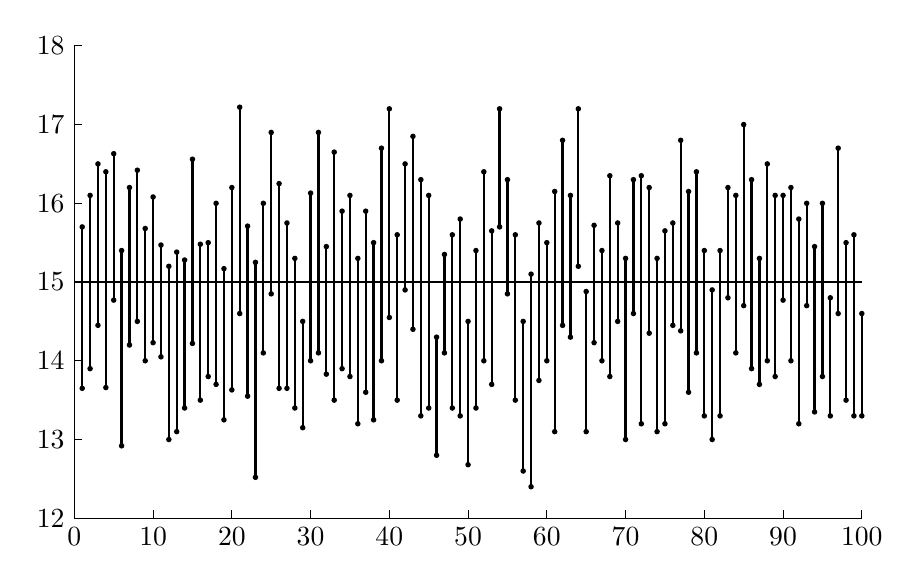
\begin{tikzpicture}[x=0.1cm]
      \draw (0,0) -- (100,0)(0,0) -- (0,6);
      \foreach \x in {0,10,...,100}
        \draw (\x,0) node[below] {$\x$} -- ++(0,0.1);
      \foreach \y in {12,...,18}
        \draw (0,\y-12) node[left]{\y}-- ++(1,0);
      \foreach [count = \i]\x/\y in {
        13.65/15.7, 13.9/16.1, 14.45/16.5, 13.66/16.4,
        14.77/16.63, 12.92/15.4, 14.2/16.2, 14.5/16.42,
        14/15.68, 14.23/16.08, 14.05/15.47, 13/15.2,
        13.1/15.38, 13.4/15.28, 14.22/16.56, 13.5/15.48,
        13.8/15.5, 13.7/16, 13.25/15.17, 13.63/16.2,
        14.6/17.22, 13.55/15.71, 12.52/15.25, 14.1/16,
        14.85/16.9, 13.65/16.25, 13.65/15.75, 13.4/15.3,
        13.15/14.5, 14/16.13, 14.1/16.9, 13.83/15.45,
        13.5/16.65, 13.9/15.9, 13.8/16.1, 13.2/15.3,
        13.6/15.9, 13.25/15.5, 14/16.7, 14.55/17.2, %40
        13.5/15.6, 14.9/16.5, 14.4/16.85, 13.3/16.3,
        13.4/16.1, 12.8/14.3, 14.1/15.35, 13.4/15.6,%48
        13.3/15.8, 12.68/14.5, 13.4/15.4, 14/16.4, %52
        13.7/15.65, 15.7/17.2, 14.85/16.3, 13.5/15.6, %56
        12.6/14.5,  12.4/15.1, 13.75/15.75, 14/15.5, %60
        13.1/16.15, 14.45/16.8, 14.3/16.1, 15.2/17.2,
        13.1/14.88, 14.23/15.72, 14/15.4, 13.8/16.35,
        14.5/15.75, 13/15.3, 14.6/16.3, 13.2/16.35, %72
        14.35/16.2, 13.1/15.3, 13.2/15.65, 14.45/15.75, %76
        14.38/16.8, 13.6/16.15, 14.1/16.4, 13.3/15.4, %80
        13/14.9, 13.3/15.4, 14.8/16.2, 14.1/16.1, %84
        14.7/17, 13.9/16.3, 13.7/15.3, 14/16.5, %88
        13.8/16.1, 14.77/16.1, 14/16.2, 13.2/15.8,
        14.7/16, 13.35/15.45, 13.8/16, 13.3/14.8,
        14.6/16.7, 13.5/15.5, 13.3/15.6, 13.3/14.6
      }
      {
        \draw[thick] (\i,\x-12) -- (\i,\y-12);
        \fill (\i,\x-12) circle(1pt) (\i,\y-12) circle(1pt);
      }
      \draw [thick] (0,3) -- (100,3);
    \end{tikzpicture}
\caption{$\mu$ 的置信水平为 $0.90$ 的置信区间}
\label{fig:6.5.1}	
\end{figure}
\begin{figure}[htbp]
\centering
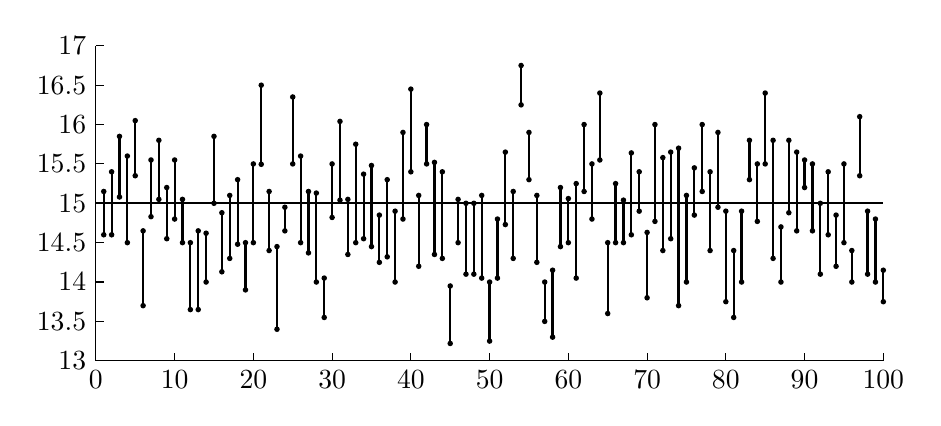
\begin{tikzpicture}[x=0.1cm]
      \draw (0,0) -- (100,0)(0,0) -- (0,4);
      \foreach \x in {0,10,...,100}
        \draw (\x,0) node[below] {$\x$} -- ++(0,0.1);
      \foreach \y in {13,13.5,14,14.5,15,15.5,16,16.5,17}
        \draw (0,\y-13) node[left]{\y}-- ++(1,0);
      \foreach [count = \i]\x/\y in {
        14.6/15.15, 14.6/15.4, 15.08/15.85, 14.5/15.6,
        15.35/16.05, 13.7/14.65, 14.83/15.55, 15.05/15.8,
        14.55/15.2, 14.8/15.55, 14.5/15.05, 13.65/14.5,
        13.65/14.65, 14/14.62, 15/15.85, 14.13/14.88,
        14.3/15.1, 14.48/15.3, 13.9/14.5, 14.5/15.5, %20
        15.495/16.5, 14.4/15.15, 13.4/14.45, 14.65/14.95,
        15.5/16.35, 14.5/15.6, 14.37/15.15, 14/15.13,
        13.55/14.05, 14.82/15.5, 15.04/16.04, 14.35/15.05,
        14.5/15.75, 14.55/15.37, 14.45/15.48, 14.25/14.85,
        14.32/15.3, 14/14.9, 14.8/15.9, 15.4/16.45, %40
        14.2/15.1, 15.5/16, 14.35/15.52, 14.3/15.4,
        13.22/13.95, 14.5/15.05, 14.1/15, 14.1/15,  %48
        14.05/15.1, 13.25/14, 14.05/14.8, 14.73/15.65,
        14.3/15.15, 16.25/16.75, 15.3/15.9, 14.25/15.1,
        13.5/14, 13.3/14.15, 14.45/15.2, 14.5/15.06,
        14.05/15.25, 15.15/16, 14.8/15.5, 15.55/16.4,
        13.6/14.5, 14.5/15.25, 14.5/15.04, 14.6/15.64,
        14.9/15.4, 13.8/14.63, 14.77/16, 14.4/15.58,
        14.55/15.65, 13.7/15.7, 14/15.1, 14.85/15.45,
        15.15/16, 14.4/15.4, 14.95/15.9, 13.75/14.9,
        13.55/14.4, 14/14.9, 15.3/15.8, 14.77/15.5,
        15.5/16.4, 14.3/15.8, 14/14.7, 14.88/15.8,
        14.65/15.65, 15.2/15.55, 14.65/15.5, 14.1/15,
        14.6/15.4, 14.2/14.85, 14.5/15.5, 14/14.4,
        15.35/16.1, 14.1/14.9, 14/14.8, 13.75/14.15
      }
      {
        \draw[thick] (\i,\x-13) -- (\i,\y-13);
        \fill (\i,\x-13) circle(1pt) (\i,\y-13) circle(1pt);
      }
      \draw [thick] (0,2) -- (100,2);
    \end{tikzpicture}
\caption{$\mu$ 的置信水平为 $0.50$ 的置信区间}
\label{fig:6.5.2}	
\end{figure}
个不包含参数真值.
在定义\ref{def:6.5.1}中使用不等式给出了区间估计的定义,实际中常用的都是等式,这便给出如下一个定义.
\end{example}

\begin{definition}{}{6.5.2}
沿用定义\ref{def:6.5.1}的记号, 如对给定的 $\alpha(0<\alpha<1)$ 对任意的 $\theta\in\Theta$, 有
\begin{equation}\label{eq:6.5.2}
P_{\theta}\left(\hat{\theta}_{L} \leqslant \theta \leqslant \hat{\theta}_{\mathrm{U}}\right)=1-\alpha
\end{equation}
则称 $\hat{\theta}_{L}$ 为 $\theta$ 的 $1-\alpha$ {\heiti 同等置信区间}\index{C!区间估计!同等置信区间}.
\end{definition}

在一些实际问题中, 人们感兴趣的有时仅仅是未知参数的一个下限或一个上限. 譬如, 对某种产品的平均寿命来说, 我们希望它越大越好, 因此人们关心的
是它的 $0.90$ 置信下限是多少, 此下限标志了该产品的质量, 它的一般定义如下.

\begin{definition}{}{6.5.3}
设 $\hat{\theta}_{L}=\hat{\theta}_{L}\left(x_{1}, \cdots, x_{n}\right)$ 是统计量, 对给定的 $\alpha\in(0,1)$ 和任意的 $\theta\in\Theta$ 有
\begin{equation}\label{eq:6.5.3}
P_{\theta}\left(\tilde{\theta}_{L} \leqslant \theta\right) \geqslant 1-\alpha, \qquad \forall \theta \in \Theta
\end{equation}
则称 $\hat{\theta}_{L}$ 为 $\theta$ 的置信水平为 $1-\alpha$ 的{\heiti (单侧)置信下限}\index{C!区间估计!(单侧)置信下限}. 假如等号对一切 $\theta\in\Theta$ 成立, 则称 $\hat{\theta}_{L}$ 为 $\theta$ 的 $1-\alpha$ {\heiti 同等置信下限}\index{C!区间估计!同等置信下限}.
\end{definition}

类似地, 对某些指标人们希望它越小越好. 比如, 某种药品的毒性, 这引出了置信上限的概念.

\begin{definition}{}{6.5.4}
设 $\hat{\theta}_{U}=\hat{\theta}_{U}\left(x_{1}, \cdots, x_{n}\right)$ 是统计量, 对给定的 $\alpha\in(0,1)$ 和任意的 $\theta\in\Theta$ , 有
\begin{equation}\label{eq:6.5.4}
P_{\theta}\left(\hat{\theta}_{U} \geqslant \theta\right) \geqslant 1-\alpha
\end{equation}
则称 $\hat{\theta}_{U}$ 为 $\theta$ 的置信水平为 $1-\alpha$ 的{\heiti (单侧)置信上限}\index{C!区间估计!(单侧)置信上限}. 若等号对一切 $\theta\in\Theta$ 成立, 则称 $\hat{\theta}_{U}$ 为 $1-\alpha$ {\heiti 同等置信上限}\index{C!区间估计!同等置信上限}.
\end{definition}

不难看出, 单侧置信下限和单侧置信上限都是置信区间的特殊情形. 因此, 寻求置信区间的方法可以用来寻找置信限. 接下来我们主要介绍寻找置信区间的方法.

\subsection{枢轴量法}\label{ssec:6.5.2}

构造未知参数 $\theta$ 的置信区间的最常用的方法是{\heiti 枢轴置法}\index{C!区间估计!枢轴置法}, 其步骤可以概括为如下三步:
\begin{enumerate}
\item 设法构造一个样本和 $\theta$ 的函数 $G=G\left(x_{1}, \cdots, x_{n}, \theta\right)$ 使得 $G$ 的分布不依赖于未知参数. 一般称具有这种性质的 $G$ 为枢轴量.
\item 适当地选择两个常数 $c$、$d$, 使对给定的 $\alpha (0<\alpha<1)$, 有
\begin{equation}\label{eq:6.5.5}
P(c \leqslant G \leqslant d)=1-\alpha
\end{equation}
\item 假如能将 $c\leqslant G\leqslant d$ 进行不等式等价变形化为 $\hat{\theta}_{L} \leqslant \theta \leqslant \hat{\theta}_{\mathrm{U}}$, 则有
\begin{equation}\label{eq:6.5.6}
P_{\theta}\left(\hat{\theta}_{L} \leqslant \theta \leqslant \hat{\theta}_{U}\right)=1-\alpha
\end{equation}
这表明 $\left[\hat{\theta}_{L}, \hat{\theta}_{v}\right]$ 是 $\theta$ 的 $1-\alpha$ 同等置信区间.
\end{enumerate}
上述构造置信区间的关键在于构造枢轴量 $G$, 故把这种方法称为{\heiti 枢轴置法}\index{C!区间估计!枢轴置法}. 枢轴量的寻找一般从 $\theta$ 的点估计出发.而满足\ref{eq:6.5.5}的 $c$、$d$ 可以有很多, 选择的目的是希望\ref{eq:6.5.6}中的平均长度 $E_{\theta}\left(\tilde{\theta}_{U}-\hat{\theta}_{L}\right)$ 尽可能短.
假如可以找到这样的 $c$、$d$ 使 $E_{\theta}\left(\tilde{\theta}_{U}-\hat{\theta}_{L}\right)$ 达到最短当然是最好的,不过在不少场合很难做到这一点.故常这样选择 $c$ 和 $d$, 使得
\begin{equation}\label{eq:6.5.7}
P_{\theta}(G<c)=P_{\theta}(G>d)=\alpha / 2
\end{equation}
这样得到的置信区间称为{\heiti 等尾置倍区间}\index{C!区间估计!等尾置倍区间}. 实用的置信区间大都是等尾置信区间.

\begin{example}
设 $x_{1}, \cdots, x_{n}$ 是来自均匀总体 $U(0, \theta)$ 的一个样本, 试对给定的 $\alpha(0<\alpha<1)$ 给出 $\theta$ 的 $1-\alpha$ 同等置信区间.
\end{example}\begin{solution}
我们采用枢轴量法分二步进行
\begin{enumerate}
\item[(1)] 我们已知 $\theta$ 的最大似然估计为样本的最大次序统计量 $x_{(n)}$, 而 $x_{(n)} / \theta$ 的密度函数为
\[p(y ; \theta)=n y^{n-1}, \qquad 0<y<1\]
它与参数 $\theta$ 无关, 故可取 $x_{(n)} / \theta$ 作为枢轴量 $G$.
\item[(2)] 由于 $x_{(n)} / \theta$ 的分布函数为 $F(y)=y^{n}, 0<y<1$, 故 $P\left(c \leqslant x_{(n)} / \theta \leqslant d\right)=d^{n}-c^{n}$, 因此我们可以适当的选择 $c$ 和 $d$ 满足
\[d^{n}-c^{n}=1-a\]
\item[(3)] 利用不等式变形可容易地给出 $\theta$ 的 $1-\alpha$ 同等置信区间为 $\left[x_{(n)} / d,x_{(n)}/c\right]$, 该区间的平均长度为 $\left(\frac{1}{\varepsilon}-\frac{1}{d}\right) E x_{(n)}$, 不难看出, 在 $0 \leqslant c<d \leqslant 1$ 及 $d^{n}-c^{n}=1-a$ 的条件下, 当 $d=1, c=\sqrt[n]{a}$ 时, $\frac{1}{c}-\frac{1}{d}$ 取得最小值, 这说明 $\left[x_{(n)},x_{(n)} / \sqrt[n]{a} \right]$ 是 $\theta$ 的置信水平为 $1-\alpha$ 最短量信区间.
\end{enumerate}
\end{solution}

\subsection{单个正态总体参数的置信区间}\label{ssec:6.5.3}

正态总体 $N(\mu,\sigma^2)$ 是最常见的分布, 本小节中我们讨论它的两个参数的置信区间.

\subsubsection{$\sigma$ 己知时 $\mu$ 的置信区间}\label{sssec:6.5.3.1}
在这种情况下, 由于 $\mu$ 的点估计为 $\bar x$, 其分布为 $N\left(\mu, \sigma^{2} / n\right)$, 因此枢轴量可选为 $G=\frac{\overline{x}-\mu}{\sigma / \sqrt{n}} \sim N(0,1)$, $c$ 和 $d$ 应满足 $P(c \leqslant G \leqslant d)=\Phi(d)-\Phi(c)=1-\alpha$, 经过不等式变形可得
\[P_{\mu}(\overline{x}-d \sigma / \sqrt{n} \leqslant \mu \leqslant \overline{x}-c\sigma\sqrt{n})=1-a\]
该区间长度为 $(d-c) \sigma \sqrt{n}$. 由于标准正态分布为单峰对称的, 从图 \ref{fig:6.5.3} 上不难看出在 $\Phi(d)-\Phi(c)=1-\alpha$ 的条件下, 当 $d=-c=u_{1-\alpha/ 2}$ 时, $d-c$ 达到最小, 由此给出了 $\mu$ 的 $1-\alpha$ 同等置信区间为
\begin{equation}\label{eq:6.5.8}
\left[\overline{x}-u_{1-\alpha / 2} \sigma / \sqrt{n}, \quad \overline{x}+u_{1-\alpha / 2} \sigma / \sqrt{n}\right]
\end{equation}
这是一个以 $\bar x$ 为中心, 半径为 $u_{1-\alpha / 2} \sigma / \sqrt{n}$ 的对称区间, 常将之表示为 $\overline{x} \pm u_{1-\alpha / 2} \sigma / \sqrt{n}$.
\begin{figure}[htbp]
\centering
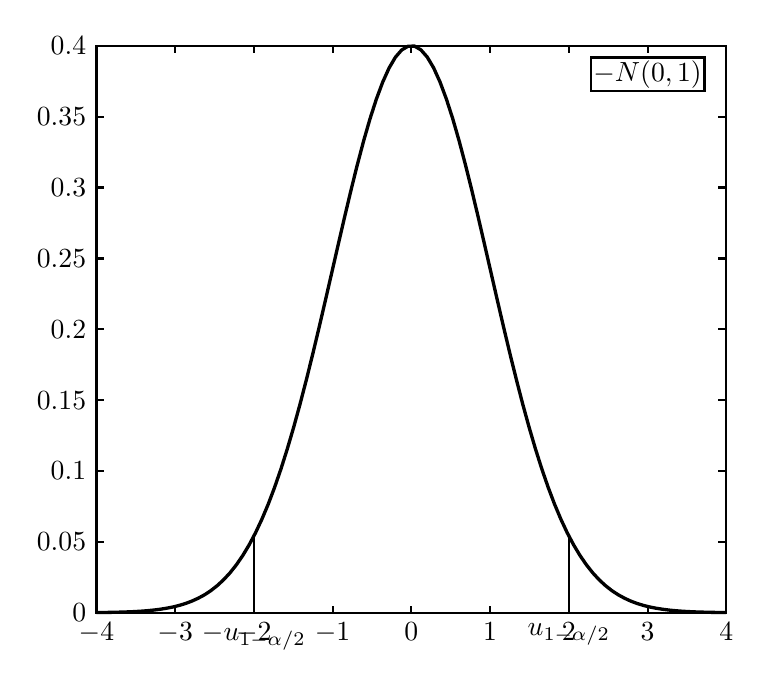
\begin{tikzpicture}[yscale=18,thick]
      \foreach \x in {-4,...,4}
        \draw (\x,0) node[below]{$\x$} -- (\x,0.005)(\x,0.4) -- (\x,0.395);
      \foreach \y in {0,0.05,0.1,0.15,0.2,0.25,0.3,0.35,0.4}
        \draw (-4,\y) node[left]{\y} -- ++(0.1,0)
              (4,\y) -- ++(-0.1,0);
      \draw (-4,0) -- (4,0) -- (4,0.4) -- (-4,0.4) -- cycle;
      \draw [very thick,domain=-4:4,samples=100] plot (\x,{0.4*e^(-(\x)^2/2)});
      \draw (-2,0) node[below=0.3] {$-u_{1-\alpha/2}$} --
      (-2,{0.4*e^(-2^2/2)})
      (2,0) node[below=0.3] {$u_{1-\alpha/2}$} --
      (2,{0.4*e^(-2^2/2)})
      (3,0.38) node [draw, inner sep = 1pt] {$-N(0,1)$};
    \end{tikzpicture}
\caption{标准正态分布示意图}
\label{fig:6.5.3}	
\end{figure}

\begin{example}\label{exam:6.5.3}
用天平称量某物体的质量 $9$ 次, 得平均值为 $\overline{x}=15.4(g)$, 已知天平称量结果为正态分布, 其标准差为 $0.1g$. 试求该物体质量的 $0.95$ 置信区间.
\end{example}\begin{solution}
此处 $1-\alpha=0.95, \alpha=0.05$, 查表知 $u_{0.975}=1.96$, 于是该物体质量 $\mu$ 的 $0.95$ 置信区间为
\[\overline{x} \pm u_{1-\alpha/ 2} \sigma / \sqrt{n}=15.4 \pm 1.96 \times 0.1 / \sqrt{9}=15.4 \pm 0.0653\]
从而该物体质量的 $0.95$ 置信区间为 $[15.3347,15.4653]$.
\end{solution}

\begin{example}\label{exam:6.5.4}
设总体为正态分布 $N(\mu,1)$, 为得到 $\mu$ 的置信水平为 $0.95$ 的置信区间长度不超过 $1.2$, 样本容量应为多大?
\end{example}\begin{solution}
由题设条件知 $\mu$ 的 $0.95$ 置信区间为
$\left[\overline{x}-u_{1-\alpha/ 2} / \sqrt{n}, \quad \overline{x}+u_{1-\alpha / 2} / \sqrt{n}\right]$
其区间长度为 $2 u_{1-{\alpha/ 2}}/\sqrt{n}$, 它仅依赖于样本容量 $n$ 而与样本具体取值无关. 现要求 $2 u_{1-\alpha / 2} / \sqrt{n} \leqslant 1.2$, 立即有 $n \geqslant(2 / 1.2)^{2} u_{1-\alpha/2}^{2}$· 现 $1-\alpha=0.95$, 故 $u_{1-\alpha / 2}=1.96$, 从而 $n \geqslant(5 / 3)^{2} \times 1.96^{2}=10.67 \approx 11$. 即样本容量至少为 $11$ 时才能使得 $\mu$ 的置信水平为 $0.95$ 的置信区间长度不超过 $1.2$.
\end{solution}

\subsubsection{$\sigma$ 未知时 $\mu$ 的置信区间}\label{sssec:6.5.3.2}

这时可用 $t$ 统计量, 因为 $t=\frac{\sqrt{n}(\overline{x}-\mu)}{s} \sim t(n-1)$, 因此 $t$ 可以用来作为 枢轴量.完全类似于上一小节, 可得到 $\mu$ 的 $1-\alpha$ 置信区间为
\begin{equation}\label{eq:6.5.9}
\left[\overline{x}-t_{1-\alpha/ 2}(n-1) s / \sqrt{n}, \overline{x}+t_{1-\alpha/ 2}(n-1) s / \sqrt{n}\right]
\end{equation}
此处 $s^{2}=\frac{1}{n-1} \sum\left(x_{i}-\overline{x}\right)^{2}$ 是 $\sigma^2$ 的无偏估计.

\begin{example}\label{exam:6.5.5}
假设轮胎的寿命服从正态分布.为估计某种轮胎的平均寿命, 现随机地抽 $12$ 只轮胎试用, 测得它们的寿命(单位: 万公里)如下:
\[\begin{array}{cccccccccccc}
4.68 & 4.85 & 4.32 & 4.85 & 4.61 &5.02 & 5.20 & 4.60 & 4.58 & 4.72 & 4.38 & 4.70
\end{array}\]
试求平均寿命的 $0.95$ 置信区间.
\end{example}\begin{solution}
此处正态总体标准差未知, 可使用 $t$ 分布求均值的置信区间. 本例中经计算有 $\overline{x}=4.7092, s^{2}=0.0615$. 取 $\alpha=0.05$, 查表知 $t_{0.975}(11)=2.2010$, 于是平均寿命的 $0.95$ 置信区间为(单位:万公里)
\[4.7092 \pm 2.2010 \cdot \sqrt{0.0615} / \sqrt{12}=[4.5516,4.8668]\]
在实际问题中, 由于轮胎的寿命越长越好, 因此可以只求平均寿命的置信下限, 也即构造单边的置信下限. 由于
\[P\left(\frac{\sqrt{n}(\overline{x}-\mu)}{s}<t_{1-\alpha}(n-1)\right)=1-\alpha\]
由不等式变形可知 $\mu$ 的 $1-\alpha$ 置信下限为 $\overline{x}-t_{1-\alpha}(n-1) s / \sqrt{n}$. 将 $t_{0.95}(11)=1.7959$ 代入计算可得平均寿命 $\mu$ 的 $0.95$ 置信下限为 $4.5806$ (万公里).
\end{solution}

\subsubsection{$\sigma^2$ 的置信区间}\label{sssec:6.5.3.3}

此时虽然也可以就 $\mu$ 是否已知分两种情况讨论 $\sigma^2$ 的置信区间, 在实际中 $\sigma^2$ 未知时 $\mu$ 已知的情形是极为罕见的, 所以我们只在 $\mu$ 未知的条件下讨论 $\sigma^2$ 的置信区间.

枢轴量不难给出. 大家知道, $\sigma^2$ 可用样本方差 $s^2$ 估计.在 \ref{sec:5.4} 中我们已经证明 $\frac{(n-1) s^{2}}{\sigma^{2}} \sim \chi^{2}(n-1)$, 由于 $\xi^2$ 分布是偏态分布, 寻找平均长度最短区间很难实现, 一般都改为寻找等尾置信区间: 把 $\alpha$ 平分为两部分, 在 $\chi^2$ 分布两侧各截面积为 $\alpha/2$ 的部分, 即采用 $\chi^2$ 的两个分位数 $\chi_{\alpha/ 2}^{2}(n-1)$ 和 $\chi_{1-\alpha / 2}^{2}(n-1)$ (见图 \ref{fig:6.5.4}), 它们满足
\[P\left(\chi_{\alpha/ 2}^{2} \leqslant \frac{(n-1) s^{2}}{\sigma^{2}} \leqslant \chi_{1-\alpha / 2}^{2}\right)=1-\alpha\]
由此给出 $\sigma^2$ 的 $1-\alpha$ 置信区间为
\begin{equation}\label{eq:6.5.10}
\left[(n-1) s^{2} / \chi_{1-\alpha / 2}^{2}(n-1),(n-1) s^{2} / \chi_{\alpha / 2}^{2}(n-1)\right]
\end{equation}
将\eqref{eq:6.5.10}的两端开方即得到标准差 $\sigma$ 的 $1-\alpha$ 置信区间.
\begin{figure}[htbp]
\centering
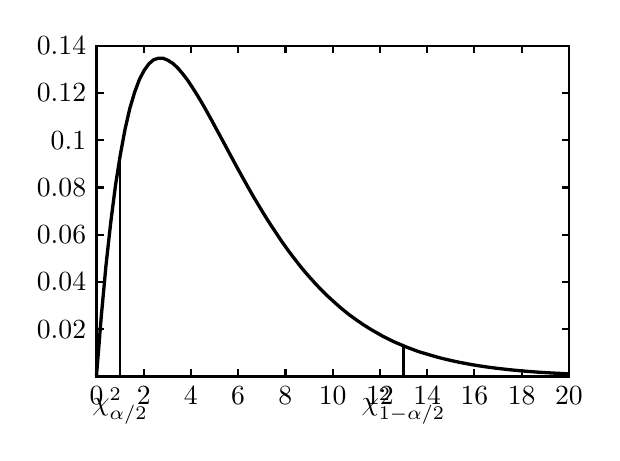
\begin{tikzpicture}[thick,yscale=30,xscale=0.3]
  \draw (0,0) -- (20,0) -- (20,0.14) -- (0,0.14) -- cycle;
  \foreach \x in {0,2,...,20}
    \draw (\x,0) node[below] {\x} -- ++(0,0.003)
    (\x,0.14) -- ++(0,-0.003);
  \foreach \y in {0.02,0.04,0.06,0.08,0.1,0.12,0.14}
    \draw (0,\y) node[left]{\y} -- ++(0.3,0)
    (20,\y) -- ++ (-0.3,0);
  \draw [very thick,domain=0:20,samples=100]
    plot(\x,{0.0045*\x*(30-\x)*e^(-\x/3)});

  \draw (1,0) node[below=0.3] {$\chi^2_{\alpha/2}$} -- (1,{0.0045*1*(30-1)*e^(-1/3)});
  \draw (13,0)node[below=0.3] {$\chi^2_{1-\alpha/2}$} -- (13,{0.0045*13*(30-13)*e^(-13/3)});

\end{tikzpicture}
\caption{$\chi^2$ 分布置信区间示意图}
\label{fig:6.5.4}	
\end{figure}

\begin{example}\label{exam:6.5.6}
某厂生产的零件重量服从正态分布 $N(\mu,\sigma^2)$, 现从该厂生产的零件中抽取 $9$ 个, 测得其质量为(单位: g)
\[\begin{array}{ccccccccc}
45.3&45.4&45.1&45.3&45.5&45.7&45.4&45.3&45.6
\end{array}\]
试求总体标准差 $\sigma$ 的 $0.95$ 置信区间.
\end{example}\begin{solution}
由数据可算得 $s^{2}=0.0325,(n-1) s^{2}=8 \times 0.0325=0.26$, 这里 $\alpha=0.05$,  查表知 $\chi_{0.025}^{2}(8)=2.1797, \chi_{0.975}^{2}(8)=17.5345$, 代入 \eqref{eq:6.5.10} 可得 $\sigma^2$ 的 $0.95$ 置信区间为
\[\left[\frac{0.26}{17.5345}, \frac{0.26}{2.1797}\right]=[0.0148,0.1193].\]
从而 $\sigma$ 的 $0.95$ 置信区间为 $[0.1218,0.3454]$.
\end{solution}

\subsection{大样本置信区间}\label{ssec:6.5.4}

在样本容量充分大时, 可以用渐近分布来构造近似的置信区间. 一个典型的例子是关于比例 $p$ 的置信区间.

设 $x_1,\cdots,x_n$ 是来自二点分布 $b(1,p)$ 的样本, 现要求 $p$ 的 $1-\alpha$ 置信区间.
由中心极限定理知, 样本均值 $\overline{x}$ 的渐近分布为 $N\left(p, \frac{p(1-p)}{n}\right)$, 因此有
\[u=\frac{\overline{x}-p}{\sqrt{p(1-p) / n}}\dot{\sim} N(0,1)\]
这个 $w$ 可作为枢轴量, 对给定 $\alpha$, 利用标准正态分布的 $1-\alpha/2$ 分位数 $u_{1-\alpha/2}$ 可得
\[P\left(\left|\frac{\overline{x}-p}{\sqrt{p(1-p) / n}}\right| \leqslant u_{1-\alpha/ 2}\right) \approx 1-\alpha\]
括号里的事件等价于
\[(\vec{x}-p)^{2} \leqslant u_{1-\alpha / 2}^{2} p(1-p) / n\]
记 $\lambda=u_{1-\alpha / 2}^{2}$, 上述不等式可化为
\[\left(1+\frac{\lambda}{n}\right) p^{2}-\left(2 \overline{x}+\frac{\lambda}{n}\right) p+\overline{x}^{2} \leqslant 0\]
左侧的二次多项式的判别式
\[\left(2 \overline{x}+\frac{\lambda}{n}\right)^{2}-4\left(1+\frac{\lambda}{n}\right) \overline{x}^{2}=\frac{4 \overline{x}(1-\overline{x})}{n}+\frac{\lambda^{2}}{n^{2}}>0,\]
故此二次多项式是开口向上并与 $x$ 轴有两个交点的曲线(见图\ref{fig:6.5.5}). 记此两个交点为 $p_L$ 和 $p_U$, 则有
\[P\left(p_{L} \leqslant p \leqslant p_{U}\right)=1-\alpha\]
\begin{figure}[htbp]
	\centering
	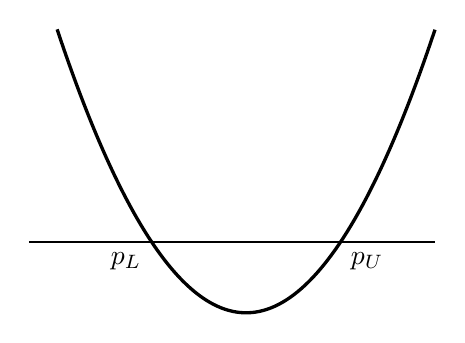
\begin{tikzpicture}[thick,xscale=1.2,yscale=0.9]
    \draw (-2.3,0) -- (2,0);
    \draw [very thick,samples=100] plot[domain=-2:2](\x,{(\x)^2-1});
    \draw (-1,0)node[below left] {$p_L$}
    (1,0) node[below right] {$p_U$};
  \end{tikzpicture}
	\caption{二次多项式及其根示意图}
	\label{fig:6.5.5}
\end{figure}
这里 $p_L$ 和 $p_U$ 是该二次多项式的两个根, 它们可表示为
\[p=\frac{1}{1+\frac{\lambda}{n}}\left(\overline{x}+\frac{\lambda}{2 n} \pm \sqrt{\frac{\overline{x}(1-\overline{x})}{n}+\frac{\lambda^{2}}{4 n^{2}}}\right)\]
由于 $n$ 比较大, 在实用中通常略去 $\lambda/n$ 项, 于是可将置信区间近似为
\begin{equation}\label{eq:6.5.11}
\left[\overline{x}-u_{1-\alpha / 2} \sqrt{\frac{\overline{x}(1-\overline{x})}{n}}, \overline{x}+u_{1-\alpha / 2} \sqrt{\frac{\overline{x}(1-\overline{x})}{n}}\right]
\end{equation}

\begin{example}\label{exam:6.5.7}
对某事件 $A$ 作 $120$ 次观察, $A$ 发生 $36$ 次. 试给出事件 $A$ 发生概率 $p$ 的 $0.95$ 置信区间.
\end{example}\begin{solution}
此处 $n=120, \overline{x}=36 / 120=0.3$, 而 $u_{0.975}=1.96$, 于是 $p$ 的 $0.95$(双侧)置信下限和上限分别为
\[\hat{p}_{L}=0.3-1.96 \times \sqrt{\frac{0.3 \times 0.7}{120}}=0.218,\]
\[\hat{p}_{U}=0.3+1.96 \times \sqrt{\frac{0.3 \times 0.7}{120}}=0.382,\]
故所求的置信区间为 $[0.218,0.382]$.
\end{solution}

\begin{example}\label{exam:6.5.8}
某传媒公司欲调查电视台某综艺节目收视率 $p$, 为使得 $p$ 的 $1-\alpha$ 置信区间长度不超过 $d_0$, 问应调查多少用户?
\end{example}\begin{solution}
这是关于二点分布比例 $p$ 的置信区间问题,由 \eqref{eq:6.5.11} 知, $1-\alpha$ 的置信区间长度为 2$u_{1-\alpha / 2} \sqrt{\overline{x}(1-\overline{x}) / n}$, 这是一个随机变量, 但由于 $\overline{x} \in(0,1)$, 所以对任意的观测值有 $\overline{x}(1-\overline{x}) \leqslant 0.5^{2}=0.25$. 这也就是说 $p$ 的 $1-\alpha$ 的置信区间长度不会超过 $u_{1-\alpha / 2} / \sqrt{n}$. 现要求 $p$ 的 $1-a$ 的置信区间长度不超过 $d_0$, 只需要 $u_{1-\alpha/2} / \sqrt{n} \leqslant d_{0}$ 即可, 从而
\begin{equation}\label{eq:6.5.12}
n \geqslant\left(\frac{u_{1-\alpha / 2}}{d_{0}}\right)^{2}
\end{equation}
这是一类常见的寻求样本量的问题. 比如, 若取 $d_{0}=0.04, \alpha=0.05$, 则
\[n\geqslant\left(\frac{u_{0.975}}{0.04}\right)^{2}=\left(\frac{1.96}{0.04}\right)^{2}=2401.\]
这表明, 要使综艺节目收视率 $p$ 的 $0.95$ 置信区间的长度不超过 $0.04$, 则需要对 $2401$ 个用户做调查.
\end{solution}

\subsection{两个正态总体下的置信区间}\label{ssec:6.5.5}

设 $x_{1}, \cdots, x_{m}$ 是来自 $N\left(\mu_{1}, \sigma_{1}^{2}\right)$ 的样本, $y_{1}, \cdots, y_{n}$ 是来自 $N(\mu_2,\sigma_2^2)$ 的样本, 且两个样本相互独立. $\overline{x}$ 与 $\overline{y}$ 分别是它们的样本均值, $s_{x}^{2}=\frac{1}{m-1} \sum_{i=1}^{m}(x_{i}-\overline{x})^2$ 和 $s_{y}^{2}=\frac{1}{n-1} \sum_{i=1}^{n}\left(y_{i}-\overline{y}\right)^{2}$. 分别是它们的样本方差. 下面讨论两个均值差和两个方差比的置信区间.

\subsubsection{$\mu_1-\mu_2$ 的置信区间}\label{sssec:6.5.5.1}

这是历史上著名的Behrens-Fisher问题, 它是Behrens在1929年从实际应用中提出的问题. 它的几种特殊情况已获得圆满的解决, 但其一般情况至今尚有学者在讨论. 下面我们对此问题分几种情况分别叙述, 读者应留意它们之间的差别及其处理方法.

1. $\sigma_1^2$ 和 $\sigma_2^2$ 已知时

此时有 $\bar x-\bar y\sim N\left(\mu_1-\mu_2,\frac{\sigma_1^2}{m}+\frac{\sigma_2^2}{n}\right)$,取枢轴量为
\[u=\frac{\bar x-\bar y-(\mu_1-\mu_2)}{\sqrt{\frac{\sigma_1^2}{m}+\frac{\sigma_2^2}{n}}}\sim N(0,1),\]
沿用前面多次用过的方法可以得到 $\mu_1-\mu_2$ 的 $1-\alpha$ 置信区间为
\[\left[\bar x-\bar y-u_{1-\alpha/2}\sqrt{\frac{\sigma_1^2}{m}+\frac{\sigma_2^2}{n}},\bar x-\bar y+u_{1-\alpha/2}\sqrt{\frac{\sigma_1^2}{m}+\frac{\sigma_2^2}{n}}\right],\]
该区间称为二样本 $u$ 区间.

2. $\sigma_1^2=\sigma_2^2=\sigma^2$ 未知时

此时有
\[\bar x-\bar y\sim N\big(\mu_1-\mu_2,\big(\tfrac{1}{m}+\tfrac{1}{n}\big)\sigma^2\big),\]
\[\frac{(m-1)s_x^2+(n-1)s_y^2}{\sigma^2}\sim\chi^2(m+n-2)\]
由于 $\bar x, \bar y, s_x^2,s_y^2$ 相互独立, 故可构造如下服从 $t$ 分布 $t(m+n-2)$ 的枢轴量
\[t=\sqrt{\frac{mn(m+n-2)}{m+n}}\frac{\bar x-\bar y-(\mu_1-\mu_2)}{\sqrt{(m-1)s_x^2+(n-1)s_y^2}}\sim t(m+n-2)\]
记 $s_w^2=\frac{(m-1)s_x^2+(n-1)s_y^2}{m+n-2}$, 则 $\mu_1-\mu_2$ 的置信区间为
\[\left[\bar x-\bar y-\sqrt{\frac{m+n}{mn}}s_wt_{1-\alpha/2}(m+n-2),\bar x-\bar y+\sqrt{\frac{m+n}{mn}}s_wt_{1-\alpha/2}(m+n-2)\right].\]

3. $\sigma_1^2/\sigma_2^2=\theta$ 已知时

此时的处理方法与2中完全类似, 只须注意到
\[\bar x-\bar y\sim N\big(\mu_1-\mu_2,\big(\tfrac{\sigma_1^2}{m}+\tfrac{\sigma_2^2}{n}\big)\sigma^2\big)=N\big(\mu_1-\mu_2,\sigma_1^2\big(\tfrac{1}{m}+\tfrac{\sigma_2^2\theta}{n}\big)\big),\]
\[\frac{(m-1)s_x^2+(n-1)s_y^2/\theta}{\sigma_1^2}=\frac{(m-1)s_x^2}{\sigma_1^2}+\frac{(n-1)s_y^2}{\sigma_2^2}\sim\chi^2(m+n-2)\]
由于 $\bar x, \bar y, s_x^2,s_y^2$ 相互独立, 仍可构造如下服从 $t$ 分布 $t(m+n-2)$ 的枢轴量
\[t=\frac{\bar x-\bar y-(\mu_1-\mu_2)}{\sqrt{(m-1)s_x^2+(n-1)s_y^2/\theta}}\sqrt{\frac{mn(m+n-2)}{m\theta+n}}\sim t(m+n-2)\]
记 $s_t^2=\frac{(m-1)s_x^2+(n-1)s_y^2/\theta}{m+n-2}$, 则 $\mu_1-\mu_2$ 的 $1-\alpha$ 置信区间为
\[\left[\bar x-\bar y-\sqrt{\frac{mn}{m\theta+n}}s_tt_{1-\alpha/2}(m+n-2),\bar x-\bar y+\sqrt{\frac{mn}{m\theta+n}}s_tt_{1-\alpha/2}(m+n-2)\right].\]

4.当 $m$ 和 $n$ 都很大时的近似置信区间

此时可以证明有
\[\frac{\bar x-\bar y-(\mu_1-\mu_2)}{\sqrt{\frac{s_x^2}{m}+\frac{s_y^2}{n}}}\sim N(0,1),\]
由此可给出 $\mu_1-\mu_2$ 的 $1-\alpha$ 近似置信区间为
\[\left[\bar x-\bar y-u_{1-\alpha/2}\sqrt{\frac{s_x^2}{m}+\frac{s_y^2}{n}},\bar x-\bar y+u_{1-\alpha/2}\sqrt{\frac{s_x^2}{m}+\frac{s_y^2}{n}}\right],\]

5.一般情况下的近似置信区间

当 $m,n$ 并不都很大时, 可采用如下的近似方法: 令 $s_0^2=s_x^2/m+s_y^2/n$, 取枢轴量
\[T=[\bar x-\bar y-(\mu_1-\mu_2)]/s_0,\]
此时 $T$ 既不服从 $N(0,1)$ 也不服从 $t$ 分布. 但研究表明它与自由度为 $l$ 的 $t$ 分布很接近, 其中 $l$ 由公式
\[l=\frac{s_0^4}{\frac{s_x^4}{m^2(m-1)}+\frac{s_y^4}{n^2(n-1)}}\]
决定, $l$ 一般不为整数, 可以取与 $l$ 最接近的整数代替之. 于是, 近似地有 $T\sim t(l)$, 从而可得 $\mu_1-\mu_2$ 的 $1-\alpha$ 近似置信区间为
\[[\bar x-\bar y-s_0t_{1-\alpha/2}(l),\bar x-\bar y+s_0t_{1-\alpha/2}(l)].\]

\begin{example}\label{exam:6.5.9}
为比较两个小麦品种的产量, 选择 18 块条件相似的试验田, 采用相同的耕作方法做试验, 结果播种甲品种的 8 块试验田的单位面积产量和播种乙品种的 10 块试验田的单位面积产量(单位:kg)分别为:
\[\begin{array}{ccccccccccc}
\text{甲品种} & 628 & 583 & 510 & 554 & 612 & 523 & 530 & 615 &     &\\
\text{乙品种} & 535 & 433 & 398 & 470 & 567 & 480 & 498 & 560 & 503 & 426
\end{array}\]
假定每个品种的单位面积产量均服从正态分布, 试求这两个品种平均单位面积产量差的置信区间(取 $\alpha=0.05$).
\end{example}\begin{solution}
以 $x_1,\cdots,x_8$ 记甲品种的单位面积产量, $y_1,\cdots,y_{10}$ 记乙品种的单位面积产量, 由样本数据可计算得到
\[\bar x=569.38,s_x^2=2140.55,m=8.\]
\[\bar y=487.00,s_y^2=3256.22,n=10,\]
下面分两种情况讨论.

  (1) 若已知两个品种单位面积产量的标准差相同, 则可采用二样本 $t$ 区间.
此处
\[s_w=\sqrt{\frac{(m-1)s_x^2+(n-1)s_y^2}{m+n-2}}=\sqrt{\frac{7\times2110.55+9\times3256.22}{16}}=52.4880,\]
\[t_{1-\alpha/2}(m+n-2)=t_{0.975}(16)=2.1199,\]
\[t_{1-\alpha/2}(m+n-2)s_w\sqrt{\frac{1}{m}+\frac{1}{n}}=2.1199\times52.4880\times\sqrt{\frac{1}{8}+\frac{1}{10}}=52.78,\]
故 $\mu_1-\mu_2$ 的 0.95 置信区间为
\[569.38-487\pm52.78=[29.60,135.16]\]

  (2) 若两个品种单位面积产量的方差不等, 则可采用近似 $t$ 区间. 此处
\[s_0^2=2110.55/8+3256.22/10=589.44,s_0=24.28,\]
\[l=\frac{589.44^2}{\frac{2110.55^2}{8^2\times7}+\frac{3256.22^2}{10^2\times11}}=17.74\approx18,\]
\[s_0t_{0.975}(l)=24.28\times2.1009=51.01\]
于是 $\mu_1-\mu_2$ 的 0.95 近似置信区间为 $[31.37, 133.38]$.
\end{solution}

\subsubsection{$\sigma_1^2/\sigma_2^2$ 的置信区间}

由于 $(m-1)s_x^2/\sigma_1^2\sim\chi^2(m-1),(n-1)s_y^2/\sigma_2^2\sim\chi^2(n-1)$ 且 $s_x^2$ 与 $s_y^2$ 相互独立, 故可仿照 $F$ 变量构造如下枢轴量:
\[F=\frac{s_x^2/\sigma_1^2}{s_y^2/\sigma_2^2}\sim F(m-1,n-1)\]
对给定的置信水平 $1-\alpha$, 由
\[P\left(F_{\alpha/2}(m-1,n-1)\leqslant\frac{s_x^2}{s_y^2}\cdot\frac{\sigma_2^2}{\sigma_1^2}\leqslant F_{1-\alpha/2}(m-1,n-1)\right)=1-\alpha\]
经不等式变形即给出 $\sigma_1^2/\sigma_2^2$ 的如下的 $1-\alpha$ 置信区间:
\[\left[\frac{s_x^2}{s_y^2}\frac{1}{F_{1-\alpha/2}(m-1,n-1)},\frac{s_x^2}{s_y^2}\frac{1}{F_{\alpha/2}(m-1,n-1)}\right]\]

\begin{example}\label{exam:6.5.10}
某车间有两台自动机床加工一类套筒, 假设套筒直径服从正态分布. 现在从两个班次的产品中分别检查了 5 个和 6 个套筒, 得其直径数据如下(单位: cm):
\[\begin{array}{ccccccc}
\text{甲班}: & 5.06 & 5.08 & 5.03 & 5.00 & 5.07 &\\
\text{乙班}: & 4.98 & 5.03 & 4.97 & 4.99 & 5.02 & 4.95
\end{array}\]
试求两班加工套筒直径的方差比 $\sigma_{\text{甲}}^2/\sigma_{\text{乙}}^2$ 的 0.95 置信区间.
\end{example}\begin{solution}
此处, $m=5,n=6$, 若取 $1-\alpha=0.95$, 则查表知
\[F_{0.025}(4,5)=\frac{1}{F_{0.975}(5,4)}=\frac{1}{9.36}=0.1068,\]
\[F_{0.975}(4,5)=7.39\]
由数据算得 $\sigma_{\text{甲}}^2=0.00037$, $\sigma_{\text{乙}}^2=0.00092$, 故置信区间的两端分别为
\[\frac{s_{\text{甲}}^2}{s_{\text{乙}}^2}\cdot\frac{1}{F_{0.975}(4,5)}=\frac{0.00037}{0.00092}\cdot\frac{1}{7.39}=0.0544,\]
\[\frac{s_{\text{甲}}^2}{s_{\text{乙}}^2}\cdot\frac{1}{F_{0.075}(4,5)}=\frac{0.00037}{0.00092}\cdot\frac{1}{0.1068}=3.7657,\]
由此可知 $\sigma_{\text{甲}}^2/\sigma_{\text{乙}}^2$ 的 0.95 置信区间为 $[0.0544, 3.7657]$.
\end{solution}

\subsection{习题}\label{ssec:6.5.6}
\begin{xiti}
\item 某厂生产的化纤强度服从正态分布, 长期以来其标准差稳定在 $\sigma=0.85$, 现抽取了一个容量为 $n=25$ 的样本, 测定其强度, 算得样本均值为 $\bar x=2.25$, 试求这批化纤平均强度的置信水平为 0.95 的置信区间.
    
\item 总体 $X\sim N(\mu,\sigma^2)$, $\sigma^2$ 已知, 问样本容量 $n$ 取多大时才能保证 $\mu$ 的 95\% 的置信区间的长度不大于 $k$.
    
\item 0.50, 1.25, 0.80, 2.00是取自总体 $X$ 的样本, 已知 $Y=\ln X$ 服从正态分布 $N(\mu,1)$.
\begin{enumerate}
  \item 求 $\mu$ 的置信水平为 95\% 的置信区间;
  \item 求 $X$ 的数学期望的置信水平为 95\% 的置信区.
\end{enumerate}

\item 用一个仪表测量某一物理量 9 次, 得样本均值 $\bar x=56.32$, 样本标准差s=0.22.
\begin{enumerate}
  \item 测量标准差. 大小反映了测量仪表的精度, 试求 $\sigma$ 的 0.95 置信区间;
  \item 求该物理量真值的 0.99 置信区间.
\end{enumerate}

\item 已知某种材料的抗压强度 $X\sim N(\mu,2)$, 现随机地抽取 10 个试件进行抗压试验,测得数据如下: 482, 493, 457, 471, 510, 446, 435, 418, 394, 469.
\begin{enumerate}
  \item 求平均抗压强度 $\mu$ 的 95\% 的置信区间;
  \item 若已知  $\sigma=30$, 求平均抗压强度 $\mu$ 的95\%的置信区间;
  \item 求 $\sigma$ 的 95\% 的置信区间.
\end{enumerate}

\item 在一批货物中随机抽取 80 件, 发现有 11 件不合格品, 试求这批货物的不合格品率的0.90置信区间.
    
\item 设 $x_1,\cdots, x_n$ 是来自泊松分布 $P(\lambda)$ 的样本, 证明: $\lambda$ 的近似 $1-\alpha$ 置信区间为
\[\left[\frac{2\bar x+\frac{1}{n}u_{1-\alpha/2}^2-\sqrt{(2\bar x+\frac{1}{n}u_{1-\alpha/2})^2-4\bar{x}^2}}{2},\frac{2\bar x+\frac{1}{n}u_{1-\alpha/2}^2+\sqrt{(2\bar x+\frac{1}{n}u_{1-\alpha/2})^2-4\bar{x}^2}}{2}\right]\]

\item 某商店某种商品的月销售量服从泊松分布, 为合理进货, 必须了解销售情况. 现记录了该商店过去的一些销售量, 数据如下:
\[\begin{array}{c|cccccccc}
\text{月销售量} & 9 & 10 & 11 & 12 & 13 & 14 & 15 & 16\\
\midrule
\text{月份数}   & 1 & 6  & 13 & 12 & 9  & 4  & 2  & 1
\end{array}\]
试求平均月销售量的0.95置信区间.

\item 设从总体 $X\sim N(\mu_1,\sigma_1^2)$ 和总体 $Y\sim N(\mu_2,\sigma_2^2)$ 中分别抽取容量为 $n_1=10, n_2=15$ 的独立样本,可计算得 $\bar x=82, s_x^2=56.5, \bar y=76,s_y^2=52.4$.
\begin{enumerate}
  \item 若已知 $\sigma_1^2=64,\sigma_2^2=49$, 求 $\mu_1-\mu_2$ 的95\% 的置信区间;
  \item 若已知 $\sigma_1^2,=\sigma_2^2$, 求 $\mu_1-\mu_2$ 的 95\% 的置信区间;
  \item 若对 $\sigma_1^2,\sigma_2^2$ 一无所知, 求 $\mu_1-\mu_2$ 的 95\% 的近似置信区间;
  \item 求 $\sigma_1^2/\sigma_2^2$ 的 95\% 的置信区间.
\end{enumerate}  

\item 假设人体身高服从正态分布, 今抽测甲、乙两地区18岁~25岁女青年身高得数据如下: 甲地区抽取10名, 样本均值1.64m, 样本标准差0.2m; 乙地区抽取10名, 样本均值1.62m, 样本标准差0.4m. 求:
\begin{enumerate}
  \item 两正态总体方差比的 95\% 的置信区间;
  \item 两正态总体均值差的 95\% 的置信区间.
\end{enumerate}
\end{xiti}



